\chapter{The CMS Electromagnetic Calorimeter}
\label{sec_ecal}
\graphicspath{{ecal/figures/}{ecal/}}


The CMS ECAL is a high-resolution, hermetic, and homogeneous electromagnetic calorimeter made of 75,848 scintillating lead tungstate crystals divided among a barrel ($|\eta| < 1.48$) and two endcaps ($1.48 < |\eta| < 3.0$) \cite{cms_tdr}, as shown in Figure \ref{fig:ecal_scheme}. 
%These crystals are characterized by fast light emission, short radiation length ($X_0 = 0.89$ cm) and small Moliere radius ($R_M = 2.10$ cm). 
The light emitted by these crystals is detected with avalanche photodiodes (APDs) in the barrel and vaccuum photontriodes (VPTs) in the endcaps. The signal readout is performed with two avalanche photodiodes (APDs) per crystal in the barrel, and one vacuum phototriode (VPT) in the endcaps. These characteristics, translated into precise energy and timing resolutions, are an invaluable tool for the CMS physics program.

\begin{figure*}[bh]
\centering 
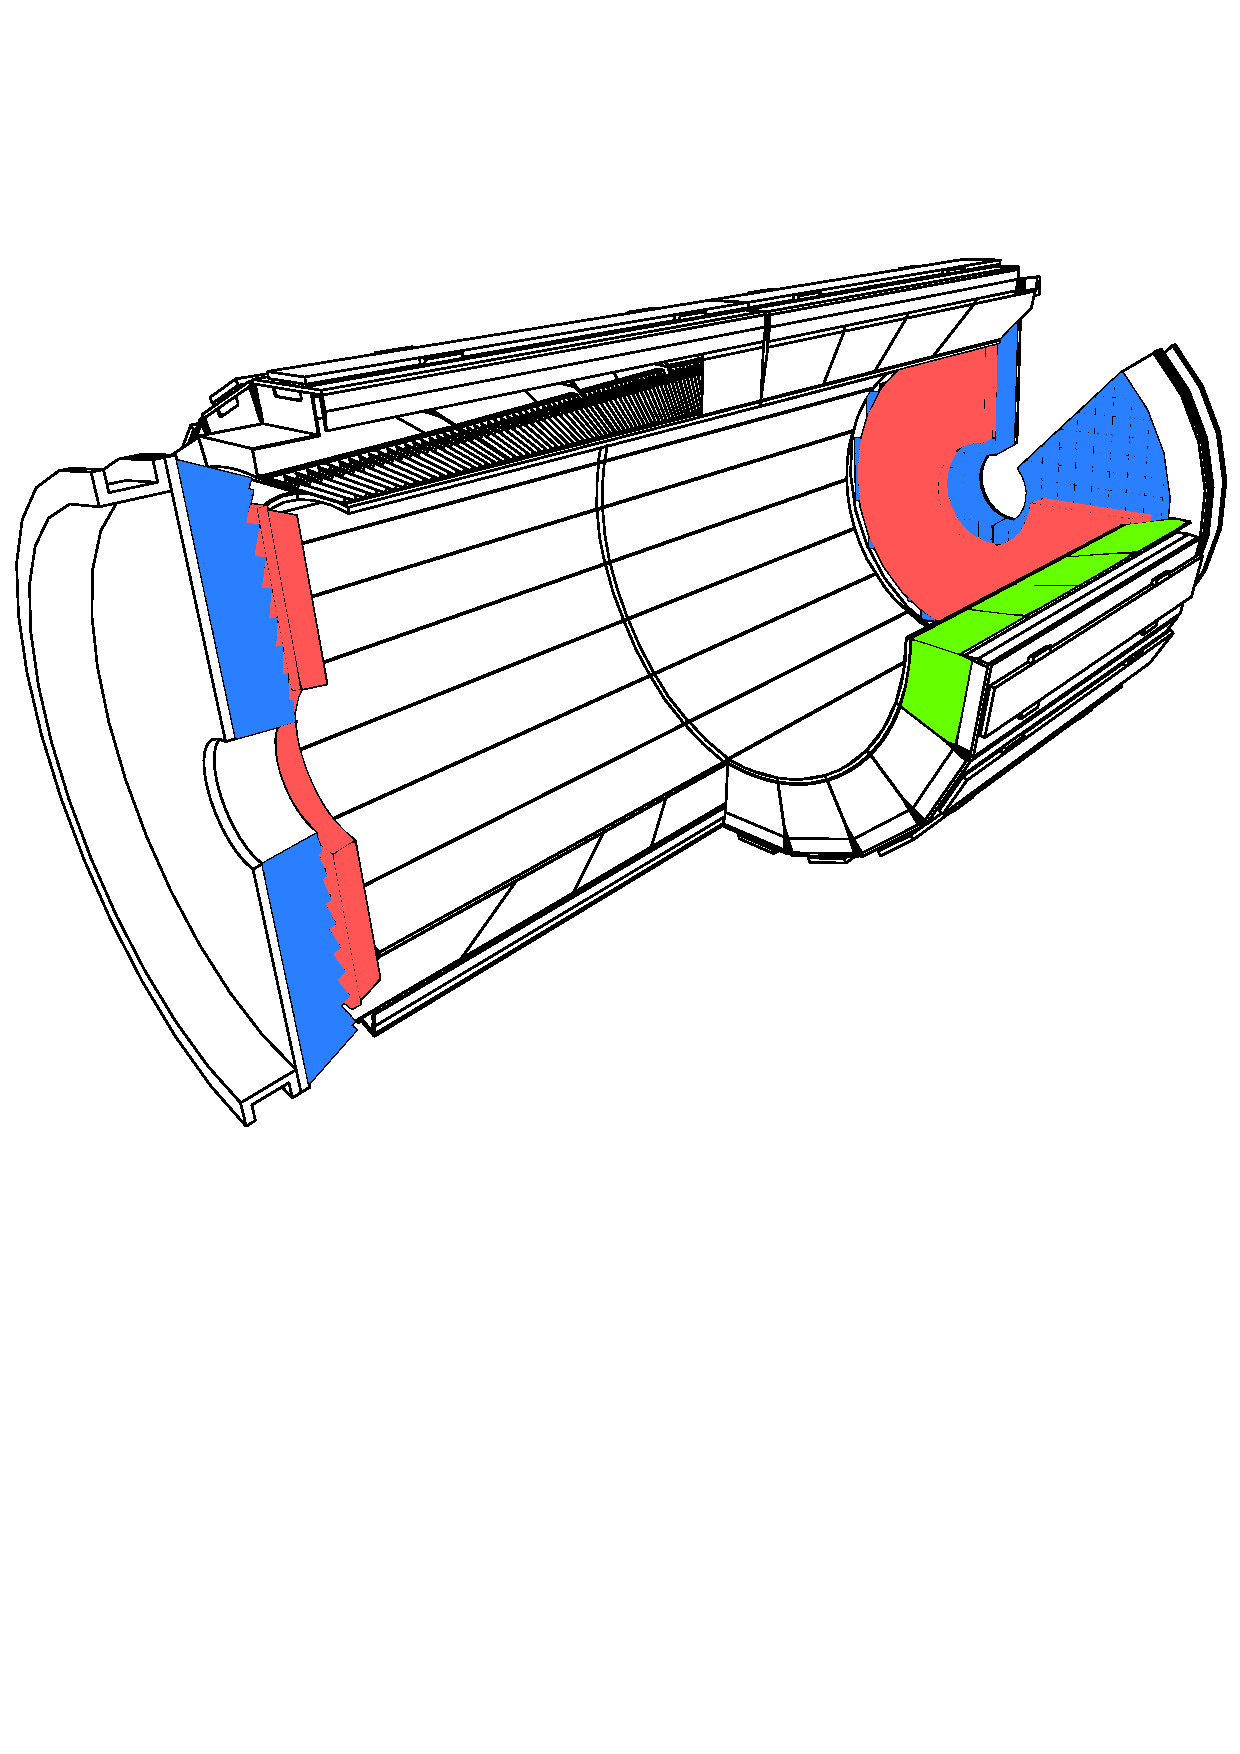
\includegraphics[width=0.7\textwidth]{figures/ECAL_scheme}\hfil
\caption{The CMS ECAL scheme highlighting a barrel supermodule (green), the ECAL endcaps (blue) and the ECAL preshower (red). }
\label{fig:ecal_scheme}
\end{figure*}


Completing the CMS electromagnetic calorimeter system is a preshower detector (ES), based on lead absorbers equipped with silicon strip sensors. It is installed in front of the ECAL endcaps, covering the region $1.65 < |\eta| < 2.6$. The fine granularity of the ES strips (2 mm wide) can resolve the signals of high-energy photons from the decays of neutral pions into two photons, when the separation angle between the photons is small, and can determine precisely the position of the electromagnetic deposits.

During the first year of Run 2 data taking at 13 TeV, the LHC provided a challenging environment, with one bunch crossing every 25 ns and an average of 10 interactions per crossing (pile up). 
The situation became even more challenging in 2016, with up to 40 pile up interactions. 
In the 2015 data taking period, the CMS ECAL operated with more than $98\%$ of its channels active, and was responsible for less than $7\%$ of CMS downtime during physics runs.


%\section{Detector Components}
\section{PbWO$_4$ Crystals and In-detector Electronics}

The main component of the ECAL are the lead tungstate crystals, that serve as both active material and absorber, constituting a homogeneous calorimeter. 
The barrel and endcap crystals are shaped as trapezoidal prisms, with 23 and 22 cm of length, respectively, consisting of about 26$X_{0}$. 
The crystal's front face (facing the interaction point) has an area of approximately $22\times22$ mm$^{2}$ (about $\Delta\eta\times\Delta\phi = 0.0175\times0.0175$) for the barrel and $25\times25$ mm$^{2}$ for the endcaps. 
Examples of such crystals are seen in Figure \ref{fig:ecal_crystals}.

\begin{figure*}[h]
\centering 
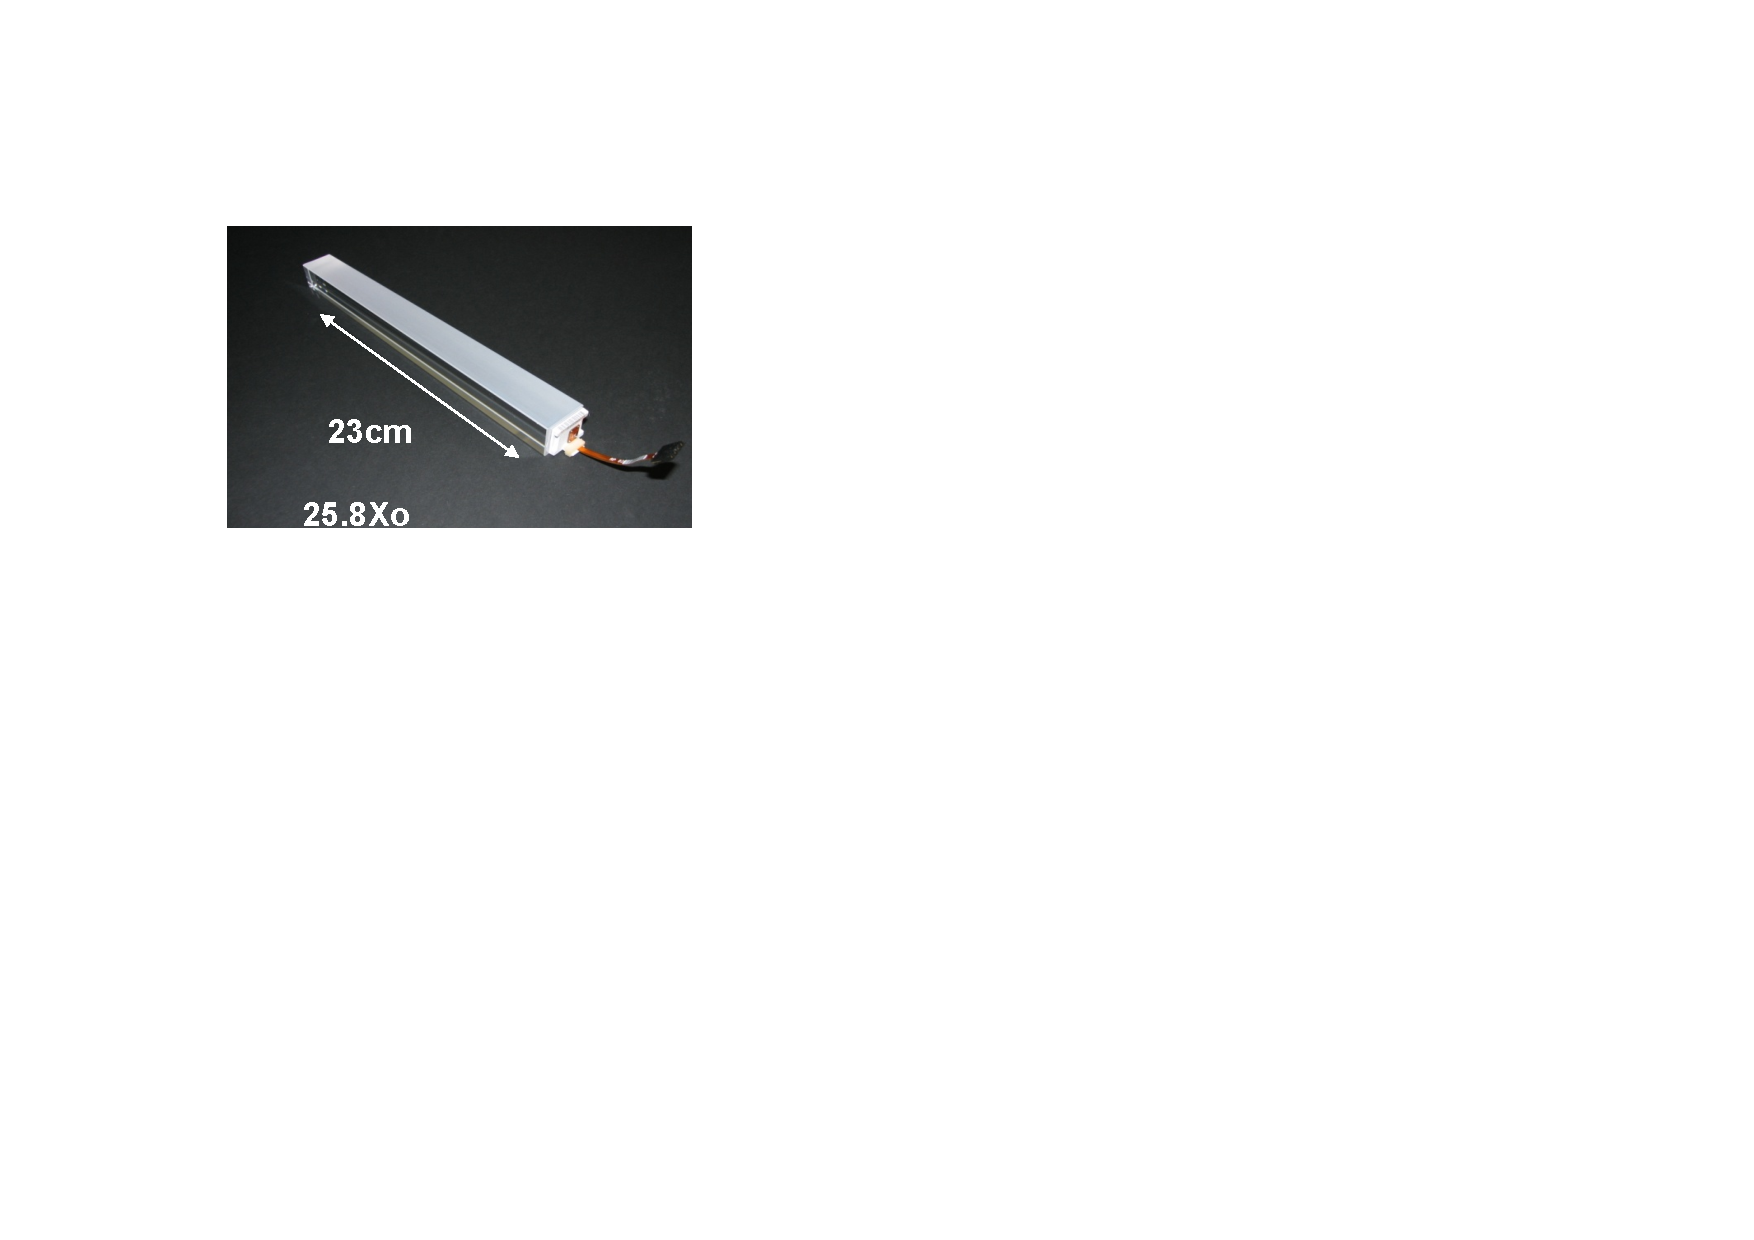
\includegraphics[width=0.45\textwidth]{figures/ecal_crystal_eb}\hfil
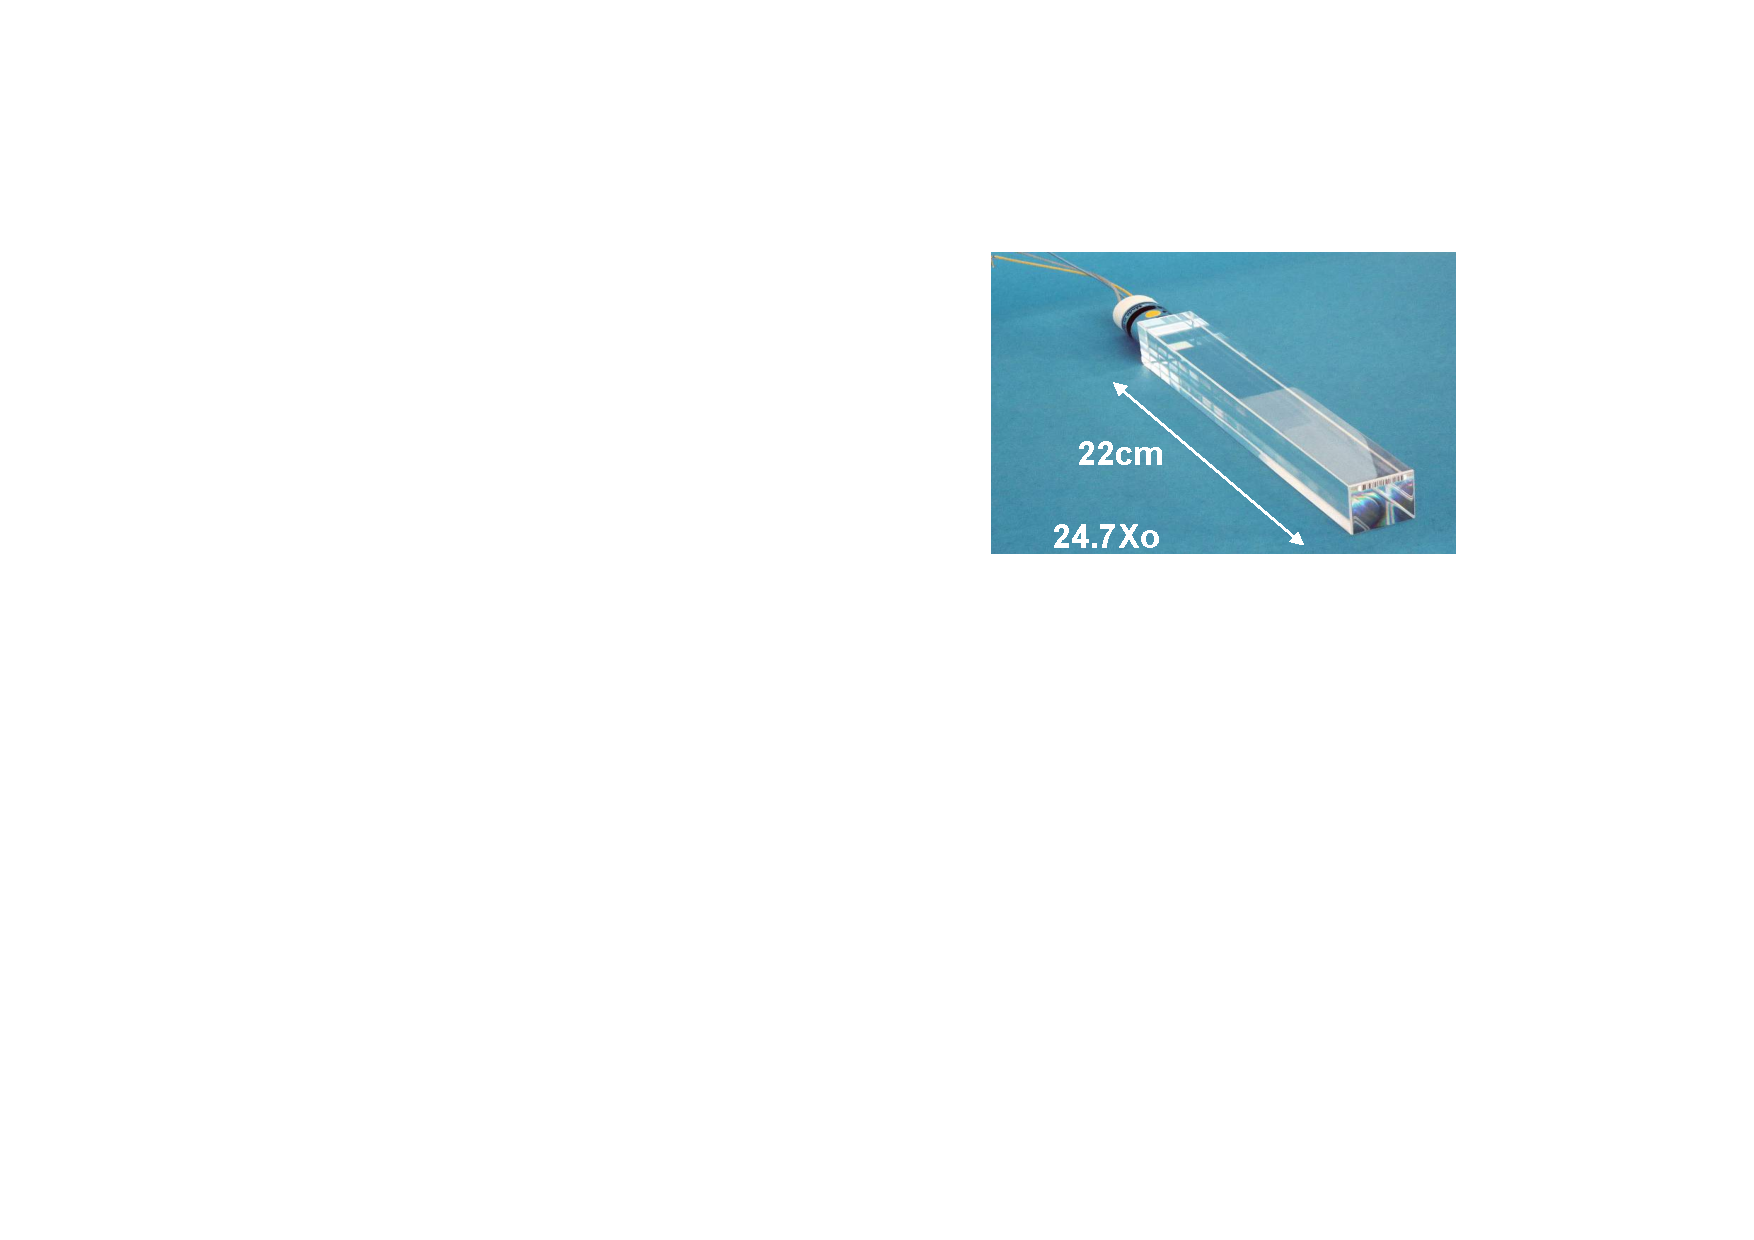
\includegraphics[width=0.45\textwidth]{figures/ecal_crystal_ee}\hfil
\caption{Example of lead tungstate crystals as present on the ECAL barrel (left) and on the ECAL endcap (right). }
\label{fig:ecal_crystals}
\end{figure*}


The ECAL crystals are arranged to provide an off-pointing, pseudo-projective geometry (the crystal axes are tilted at $3^{o}$ with respect to the line from the nominal vertex position), shown in the left of Figure \ref{fig:ecal_geometry}. 
In the barrel, the crystals are mounted in submodules ($2\times5$ crystals in $\phi\times\eta$), which are then mounted into modules and grouped into supermodules. 
Each supermodule contains 4 modules, three with $10\times4$ submodules in $\phi\times\eta$ and one with $10\times5$. An ECAL supermodule is shown on the right of Figure \ref{fig:ecal_geometry}. 

\begin{figure*}[h]
\centering 
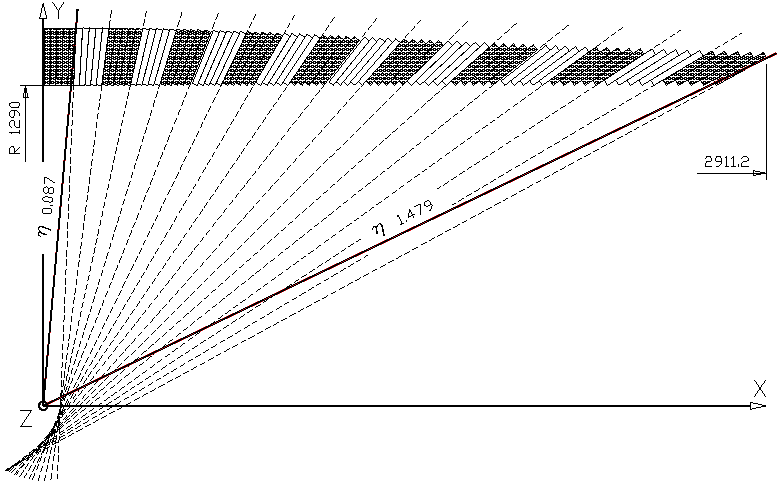
\includegraphics[width=0.45\textwidth]{figures/geometry_barrel}\hfil
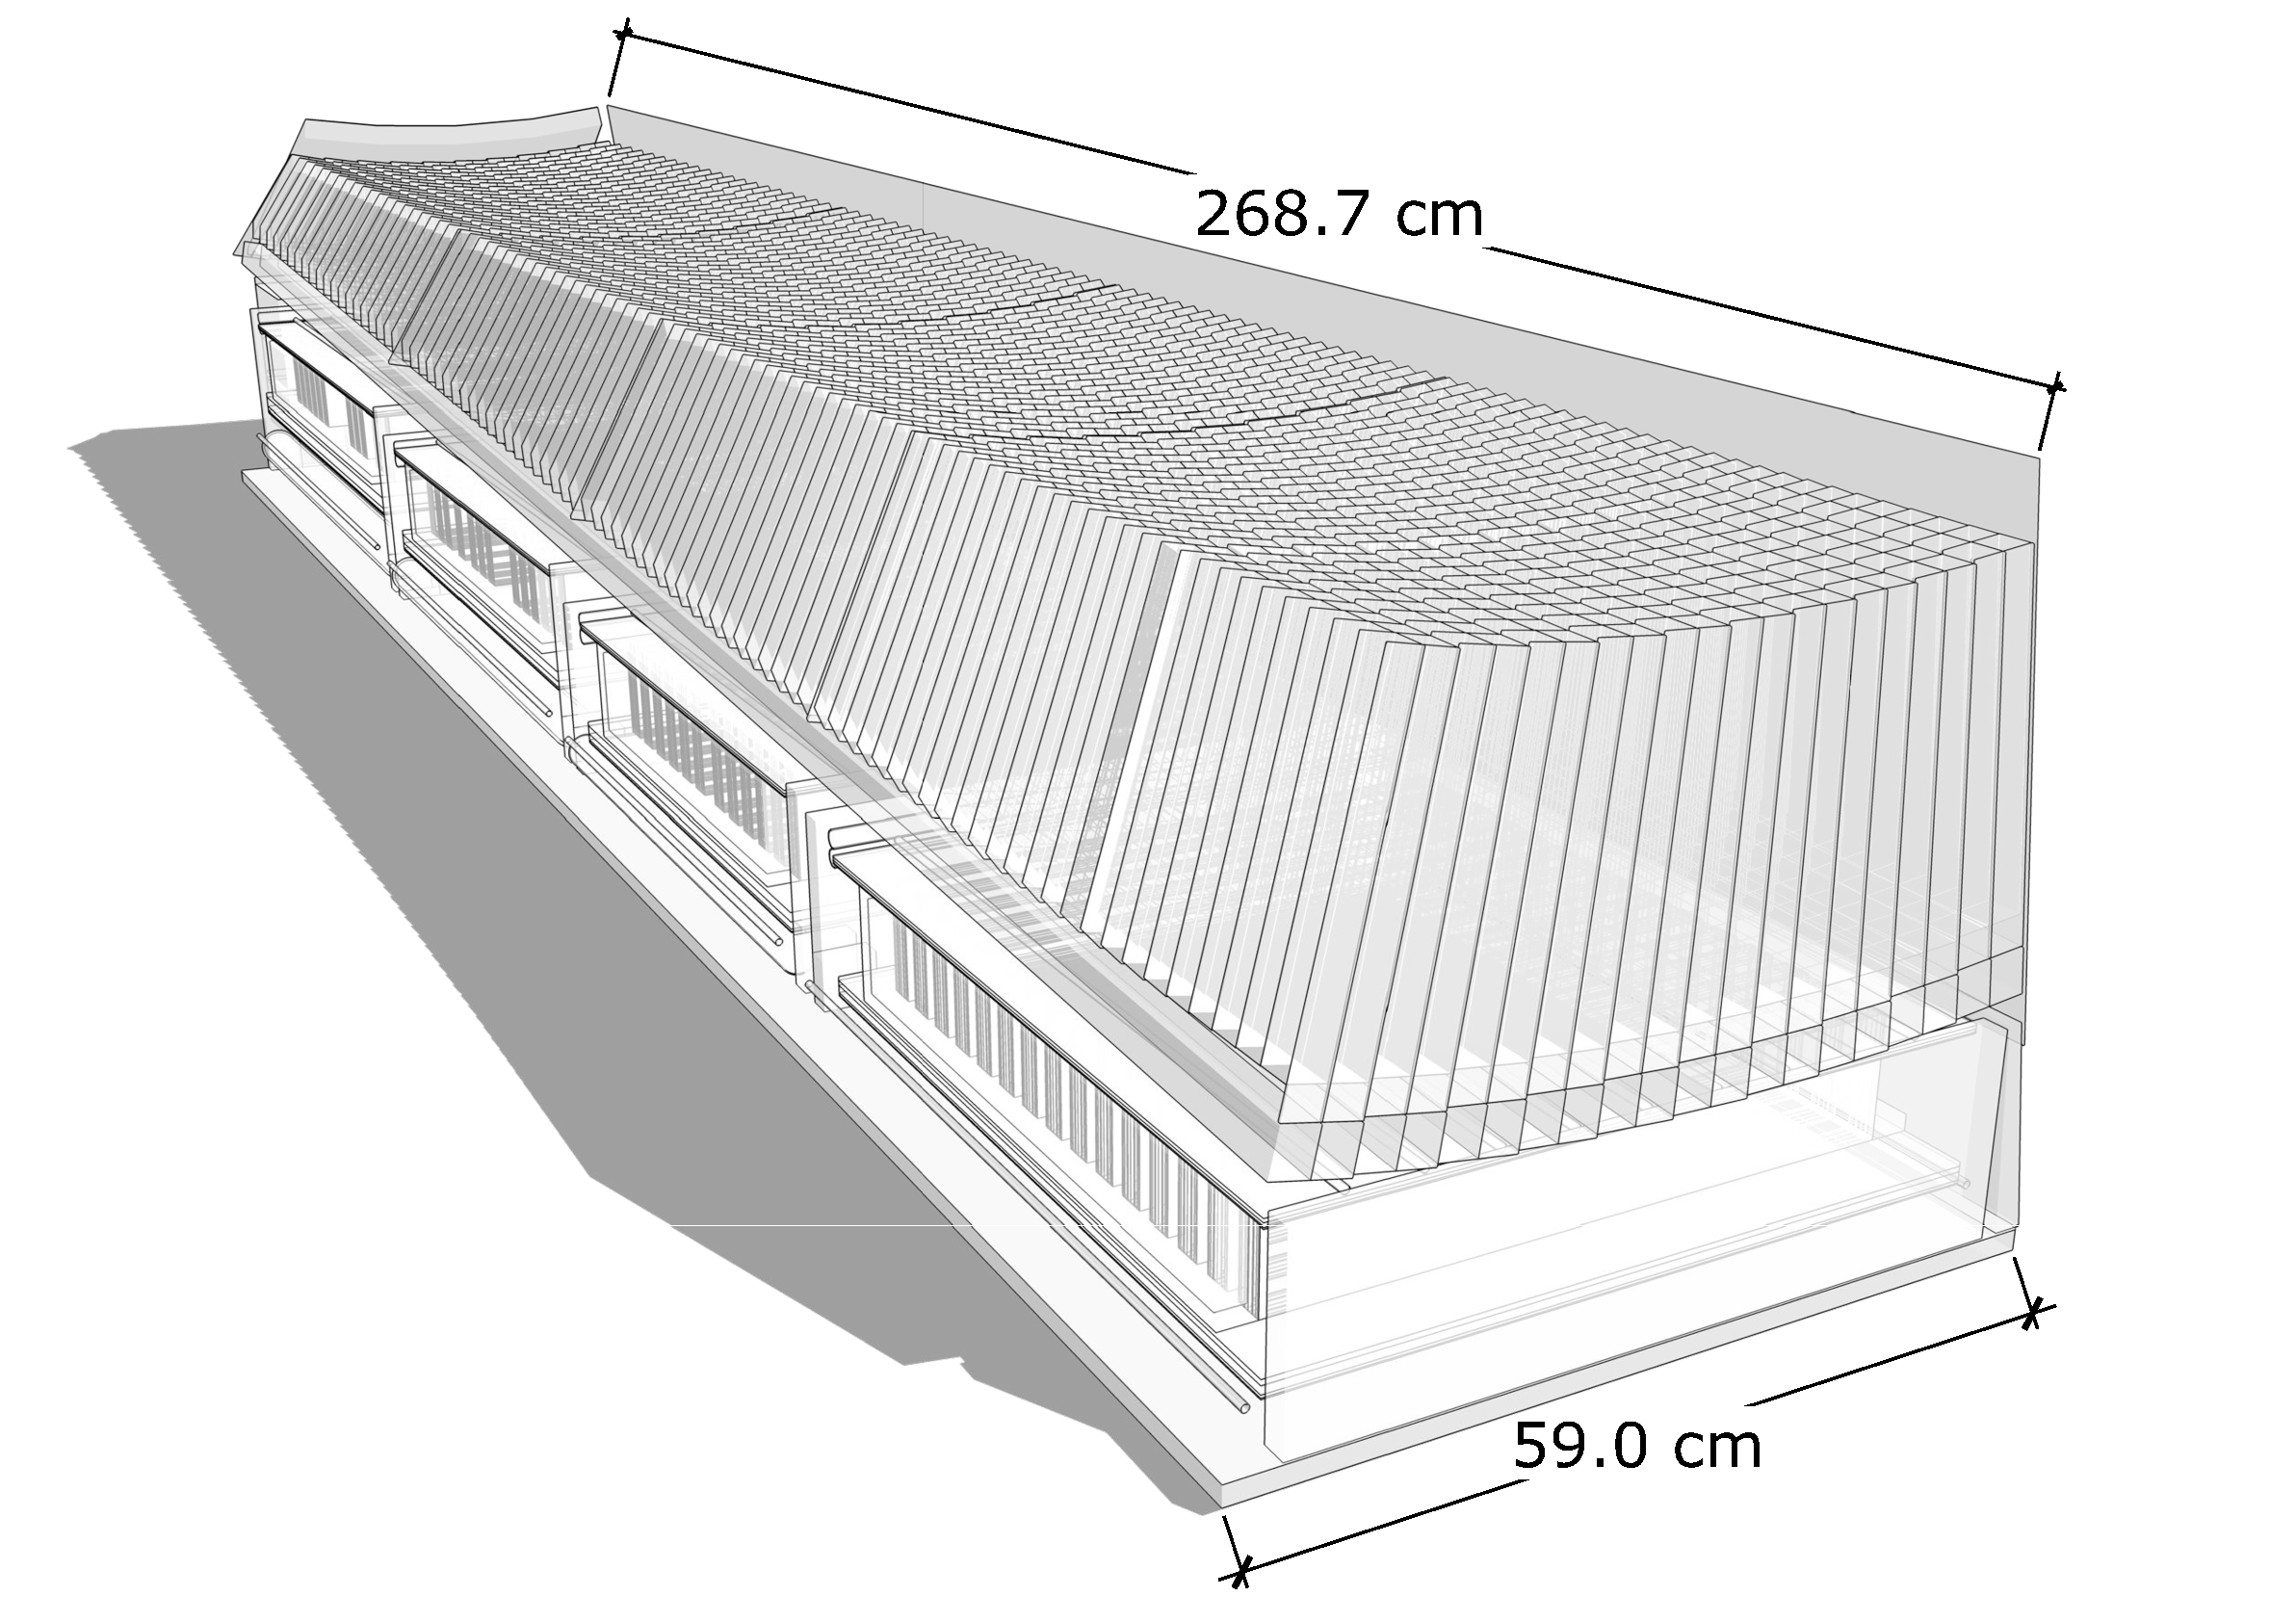
\includegraphics[width=0.45\textwidth]{figures/supermodule}\hfil
\caption{On the left, the CMS ECAL scheme highlighting a barrel supermodule (green), the ECAL endcaps (blue) and the ECAL preshower (red). On the right, the details of a barrel supermodule structure. }
\label{fig:ecal_geometry}
\end{figure*}

An energy deposit is measured in the crystal through a scintillation process, in which the lattice atoms are excited and de-excite by the emission of photons. 
The emission scintillation peak for the ECAL crystals is at about $425$ nm, with $80\%$ of the light emission happening within 25 ns. 
The PbWO$_4$ crystals are also characterized by a small radiation length ($X_{0} = 0.89$ cm), the mean length of the path that takes a high energy electron to lose $(1 - 1/e)$ of its energy in that medium, and a small Moli�re radius ($R_{M} = 2.19$ cm), the radius of a cylinder that contains $90\%$ of the shower energy. 

On the other hand, the ECAL crystals have a low light output yield (about 30 photo-electrons per MeV), and therefore must be coupled to high gain light detectors. 
These detectors must also be radiation hard, to cope with the LHC environment, and be stable under a 4T magnetic field (the CMS solenoid magnet). 
For the ECAL barrel, avalanche photodiodes (APDs) were chosen due to their high gain (50), despite their temperature dependence, which requires ECAL to have a temperature control with a precision better than $0.1^{o}$C (the PbWO$_4$ crystals light yield is also dependent on temperature, with lower light yields for lower temperatures). 

The ECAL APDs are also characterized by their fast, 2 ns rise time, which allows time measurement with the crystals scintillation pulse shape. 
By the time of the ECAL construction, APDs were generally produced in small sizes in comparison to the crystal's rear side area, where they must be attached. For this, two APDs were used for each crystal. 
On the endcaps, the radiation dose incoming is much higher than in the barrel, which does not allow the usage of APDs in the high $\eta$ region. For this reason, vacuum photo-triodes (VPTs) are used instead. While more resistant to radiation, these light detectors have generally a smaller gain (8-10).

\section{Trigger and Data Acquisition Systems}

The ECAL trigger and data acquisition system (Trigger and DAQ) takes care of the the entire data flow from the crystals to the central CMS Trigger and DAQ systems, a schematic version of the system is shown in Figure \ref{fig:ecal_daq}. 

\begin{figure*}[h]
\centering 
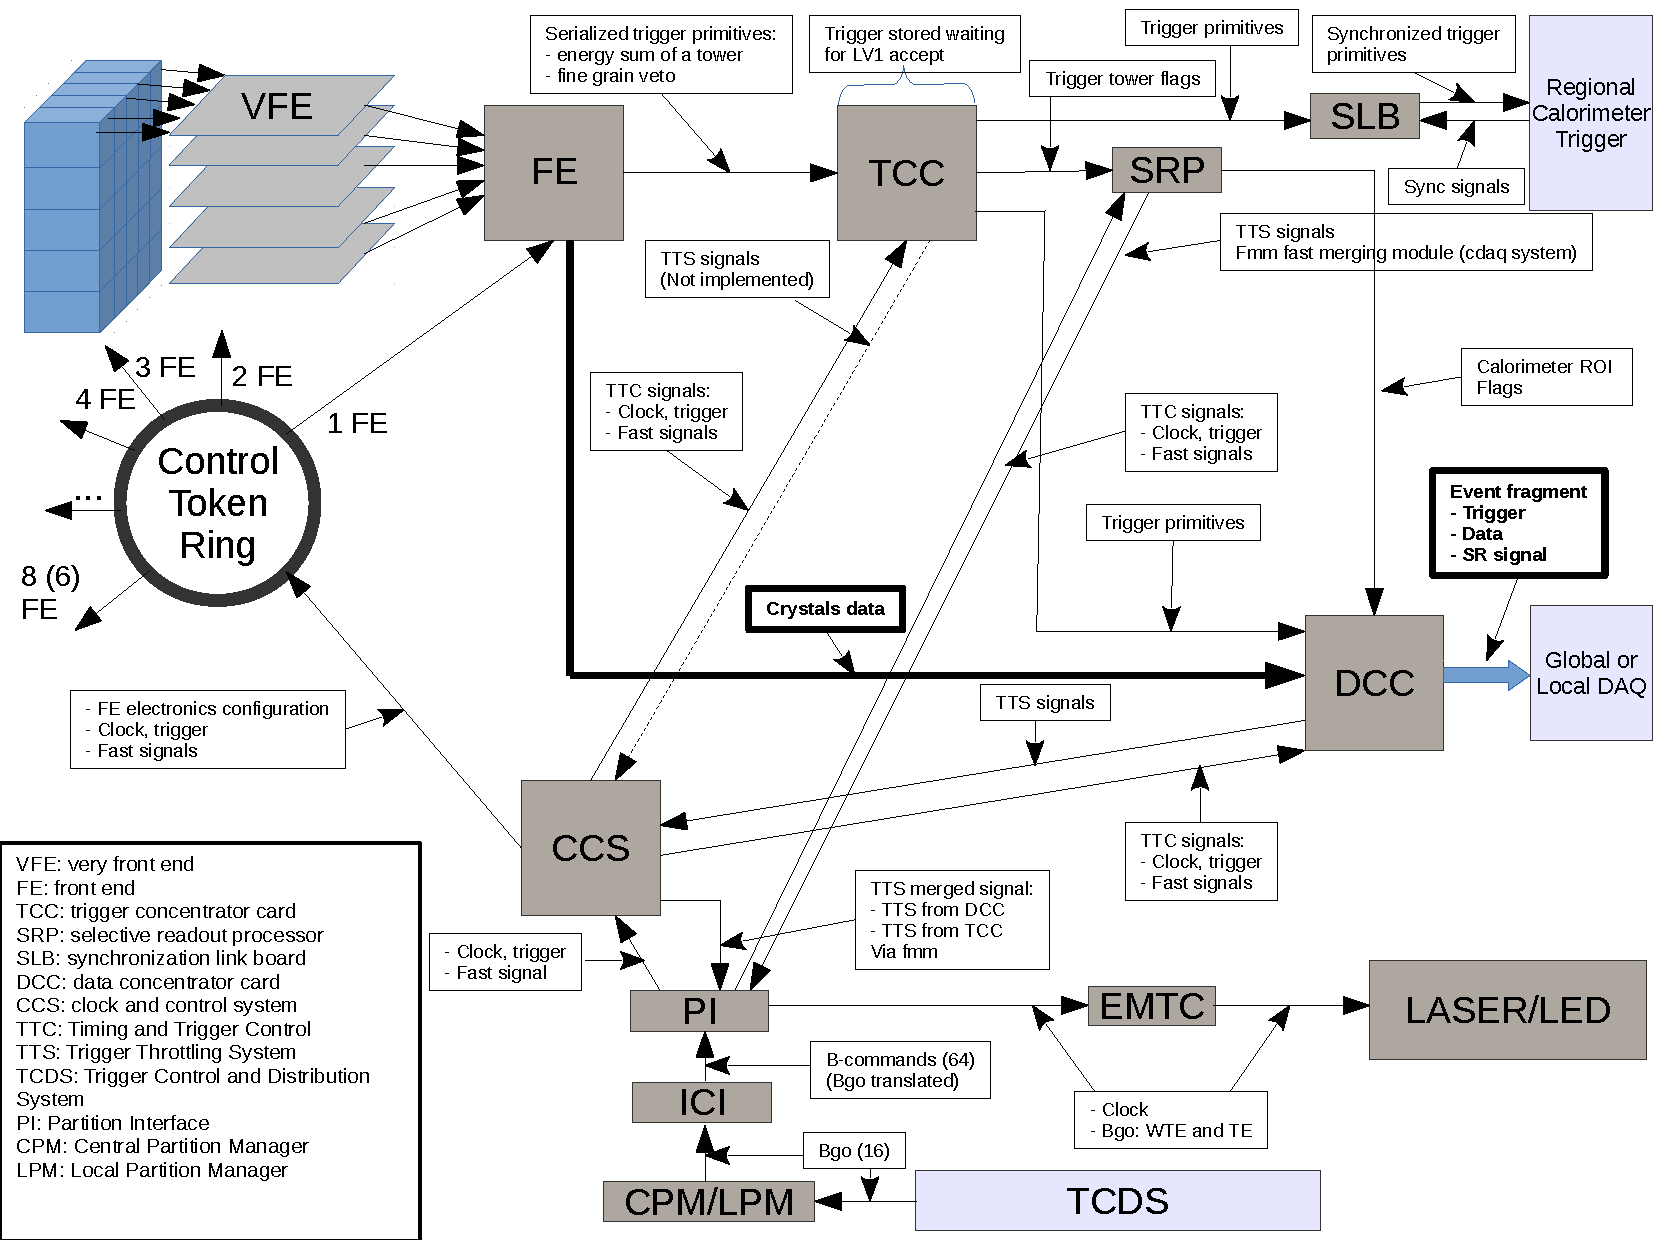
\includegraphics[width=0.7\textwidth]{figures/ecal_daq}\hfil
\caption{ECAL DAQ simplified scheme. }
\label{fig:ecal_daq}
\end{figure*}

\subsection{Data Flow}

The ECAL data flow starts right after the signal is detected by the photo detectors attached to the crystals. 
The first step in the chain is the amplification and digitization of the analog signal coming from the APDs and VPTs. 
This is performed with multi-gain pre-amplifiers (MGPAs). 
The ECAL MGPAs work with three amplification gains: gain-12, gain-6 and gain-1. 
The shaping time associated with this amplification process is of about 40 ns. 
The signal is then sampled and digitized at a rate of 40 MHz. 
One pulse shape is then reconstructed using 10 of these samples. 
The electronics responsible for the amplification and digitization step is generally called very-front-end electronics (VFE). 


The VFE sends information to the front-end electronics (FE) at the sampling rate. 
The FE is responsible for creating trigger primitives, basic information such as energy and position, from arrays of $5\times5$ crystals (trigger towers). 
The trigger primitives are sent from the FE to the trigger concentrator cards (TCCs) at sampling rate, and passed to the first layer of the CMS Level-1 trigger. 
The VFE and the FE, known as the in-detector electronics, are placed right at the detector, close to the crystals, which is schematically shown in Figure \ref{fig:ecal_vfe}. 
In Figure \ref{fig:ecal_vfe}, the chips dedicated to generating and transmitting the serialized trigger primitives (FENIX chips) are shown, along with the gigabit optical hybrids (GOH) chips dedicated to data transmission and the chips dedicated to receiving and distributing timing and control data (CCU). 

\begin{figure*}[h]
\centering 
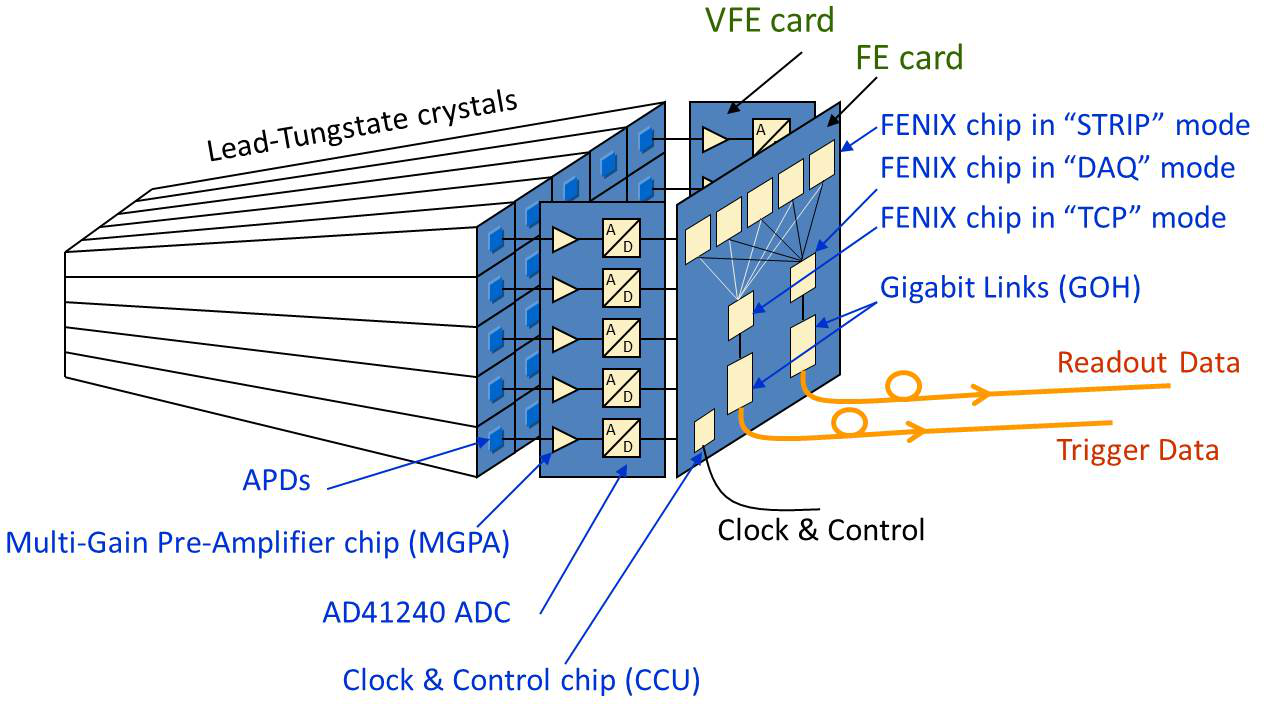
\includegraphics[width=0.7\textwidth]{figures/ecal_vfe}\hfil
\caption{ECAL in-detector electronics simplified scheme. }
\label{fig:ecal_vfe}
\end{figure*}

During the time it takes for a decision to be made by the L1 trigger (L1A signal) and to arrive back at the ECAL electronics, the trigger primitives are stored at the TCCs. 
In case the event is not accepted, these trigger primitives and the full crystal information stored at the FE are flushed from memory. 
If an event is accepted, the FE sends the serialized full individual crystals information to the data concentrator cards (DCCs), that will pack the event in a format readable by the CMS central DAQ. 

In parallel, the TCC sends the trigger primitive information to the selective readout units (SRPs) after an L1A arrives. 
The SRP selects which portions of the detector should be unpacked by the DCCs based on an algorithm called Selective Readout (SR), reducing the load of processing by the DCCs. 
The DCCs load is limited by the current electronics architecture and can be trespassed when the average activity per event is increased, such as in high pile up LHC runs.  
The SR algorithm classifies trigger towers as low interest ($E_{TT} < 1.5$ GeV), medium interest ($1.5 < E_{TT} < 2.5 $ GeV) or high interest ($E_{TT} > 2.5$ GeV). 
If a trigger tower is classified as low interest, only the crystals with energy higher than 4.5 (6.5) ADC in the barrel (endcap) are unpacked. 
If a trigger tower is classified as medium interest, all crystals are unpacked, regardless of their energies. 
If a trigger tower is classified as high interest, all crystals in that trigger tower, and the 8 trigger towers around it are fully read.

\subsection{Timing and Control Distribution}

In order to ensure a synchronized working of all different parts of the ECAL DAQ system, a precise distribution of clock and control signals must be achieved. 
This is performed via a combination of different ECAL and central CMS electronics. 
For Run 2, CMS installed a new subsystem dedicated to distributing these signals among all CMS partitions, the Timing and Control Distribution System (TCDS). 
TCDS communicates timing/synchronization signals coming from the LHC and CMS (clock), L1As coming from the CMS Level-1 trigger, and configuration and control commands synchronously to all CMS components. 
These signals are then distributed among ECAL components via the clock and control system (CCS), including to the front-end electronics (through control token rings). 

\subsubsection{TCDS}

The TCDS subsystem was installed on CMS during the Long Shutdown 1 in order to cope with the new running conditions for Run 2. 
Specifically, new detector subsystems were being installed in the experiment (such as the new pixel inner tracker layers). 
Instead of expanding the old system, a choice was made to construct a new infrastructure with updated hardware, firmware and software. 
The TCDS system consists on three types of boards: the Central Partition Manager (CPM), the CMS Interface boards (iCI) and the Partition Interface boards (PI). 

The TCDS CPM is fully controlled by the central TCDS system, and has information regarding the type of runs to be started by the central DAQ. 
This information defines, for example, at which point of the LHC orbit to send specific signals to the subdetectors. 
The iCIs must work as a library that translates the CPM signals into specific actions to be taken by the different subdetectors. This means that the iCIs must be configured properly and individually by each subdetector. 
In order to achieve that on ECAL, a new software interface to TCDS was written to configure and monitor the ECAL iCIs. 
The PIs act as fan-out boards to distribute the iCI messages among different subdetector components.

\subsection{Software Architecture}

The ECAL DAQ software architecture controls, configures and monitors the readout and trigger electronics described in the previous sections. 
The framework implementation is based on a CMS common framework developed by the central Trigger and DAQ group, mostly consisting of  C++ xDAQ framework \cite{cms_xdaq}, while the top layer of the system is based on the JAVA RCMS \cite{cms_rcms} framework.

The overall system accomplishes several different tasks. It configures and monitors the different components of the FE and and off-detector electronics. 
It communicates with the central CMS TCDS, both sending the correct configuration parameters for the dedicated TCDS ECAL boards and receiving and translating these commands to the off-detector electronics. 
It is also able to perform different types of runs dedicated to calibration and detector developments, such as "MiniDAQ" and "local" runs.

With the xDAQ framework, the ECAL software communicates to the ECAL boards through SOAP (Simple Object Access Protocol) messages. 
SOAP messages are also used to communicate issues with the off-detector electronics directly to the central DAQ system. 

There are five main components to the ECAL DAQ software architecture:
\begin{description}

\item[ECAL Function Manager] Function managers (FM) work as the overall controller of actions happening to the ECAL software. It has the power to send commands to the ECAL supervisor to cause state transitions, triggering actions such as the beginning of a run. During global CMS runs, the central DAQ function manager communicates such actions to the ECAL function manager. In specific runs in which ECAL controls its own sequence, the ECAL function manager works by itself, and can be controlled via a web interface.

\item[ECAL Supervisor] The ECAL supervisor is at the top of software control chain and coordinates all other working pieces. It receives the commands from the ECAL function manager and, to any given command, proceeds with the specific steps to ensure the state transitions of the different com ECAL components.

\item[Services Supervisors] For each different services described in the previous sections (TCC, DCC, DCS and SRP), a dedicated software exists in order to perform the actions related to specific state transitions.
\item[TCDS Supervisor] A specific supervisor was developed to communicate with the central TCDS service. It sends the proper configuration parameters to the TCDS ECAL boards, with the list of commands to be passed to the ECAL electronics when certain state transitions happen and during specific run conditions.
\item[Monitoring Services] In order to retrieve and display information about the status of the off-detector electronics, specific services based on xDAQ capabilities are used. These services also monitor the ECAL DAQ computing capabilities to make sure all machines are working properly. Depending on what type of error is detected by the monitoring services, SMS's and e-mails are sent to ECAL DAQ experts.
\end{description}

\subsubsection{ECAL DAQ Finite State Machine}

One of the main goals of the ECAL Supervisor is to ensure the proper state transitions of the different DAQ components through the allowed states of the ECAL DAQ Finite State Machine (FSM), summarized in Figure \ref{fig:ecal_fsm}.

\begin{figure*}[h]
\centering 
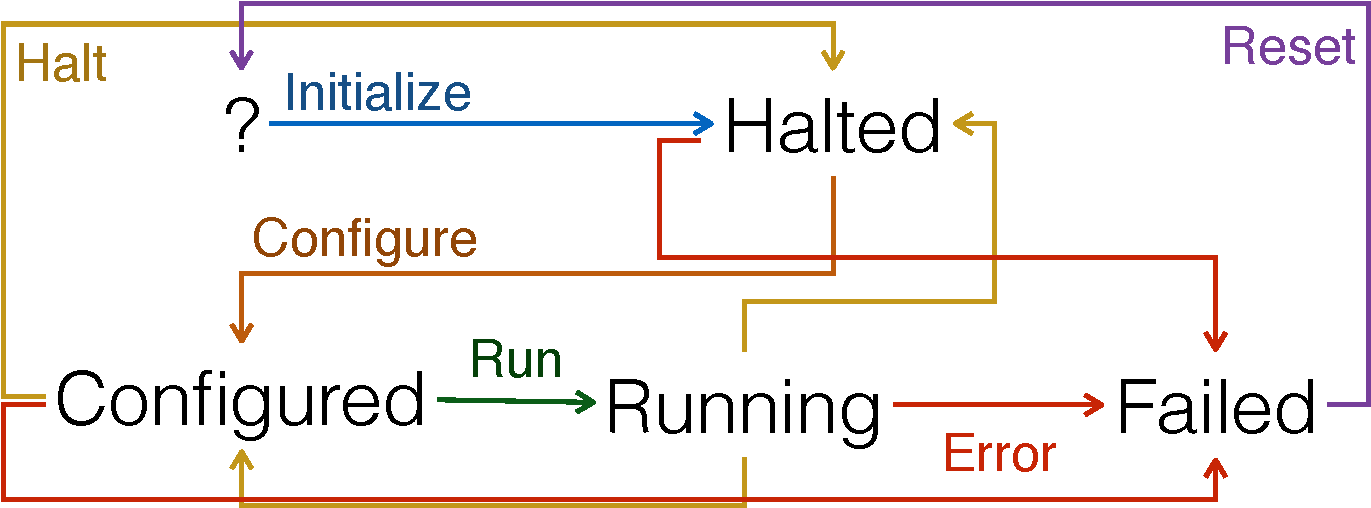
\includegraphics[width=0.7\textwidth]{figures/ecal_fsm}
\caption{Simplified view of the ECAL Finite State Machine and its transitions. }
\label{fig:ecal_fsm}
\end{figure*}

 
Similarly to the central DAQ FSM, the transitions are: 

\begin{description}
\item[Initialization] The Initialization procedure tests the connection between the ECAL Supervisor and the different off-detector components and initializes all required drivers. The information about the hardware resources is then propagated back to the supervisor and the ECAL FM. The initialization transition takes the FSM to Halted state and makes it ready to be configured.
\item[Configuration] When the configuration signal is received, it reads the configuration parameters from the ECAL Configurations DataBase (ConfDB) and sends to the off-detector electronics, which are then loaded accordingly. Each different Service Supervisor independently ensures their components have been successfully configured and communicate it back to the ECAL Supervisor. This action takes the FSM to Configured state and is now ready to start producing data (running). It also enables the monitoring services. 
\item[Start] The start command kicks-off the full data flow described at the beginning of this section, including trigger primitive production and delivery to the L1 trigger, and the delivery of the full data information upon an L1A. It also starts the delivery of monitoring data from the off-detector electronics to the monitoring services. This action takes the FSM to Running state.
\item[Stop/Halt] These actions take the system either from Running state to Configured state, or from Running or Configured states to Halted state, respectively. The Stop command  interrupts the ECAL DAQ data flow, while the the Halt command interrupts the data flow and flushes the database parameters from the off-detector electronics. 
\item[Error] Any error during the previous transitions will take the FSM to Failed state.
\end{description}

\subsubsection{Types of Running Conditions with the ECAL}

\begin{description}
\item[Global Runs] A global run is the usual working condition of ECAL with the full CMS central DAQ infrastructure. In global runs, the ECAL FM receives commands directly from the central DAQ FM, including all state transition actions. These runs happen when the LHC is running, when CMS is taking cosmics data (with its magnetic field on or off) or when specific tests must be performed with the full central DAQ infrastructure. 
\item[MiniDAQ Runs] These runs happen with a dedicated central DAQ infrastructure that is independent of global runs, and therefore can run in parallel. They are used on ECAL to test the state of the off-detector electronics and investigate possible errors seen in global runs. MiniDAQ runs have also been used in 2015 and 2016 to measure the response of the ECAL electronics to noise (pedestals) and to test pulses generated by the on-detector electronics.
\item[Local Runs] Local runs are completely independent from the central DAQ infrastructure. They rely on ECAL software to both directly configure the off-detector electronics and process the data that is produced by the DCCs. This freedom allows for more complex types of running conditions, such as the ones needed for more coherent measurements of ECAL pedestals (to be used in 2017).
\end{description}


\section{Electron and Photon Energy Reconstruction}

The photon and electron energy reconstruction based on ECAL energy deposits is based on the formula: 
\begin{equation}
E_{e,\gamma} = \left[ \sum_{i}\left( S_i(t)\times c_{i} \times A_{i}\right)\times G(\eta) + E_{ES} \right]\times F_{e,\gamma},
\end{equation}
 with $A_{i}$, $c_i$ and $S_i(t)$ as, respectively, the per individual channel amplitude, intercalibration constant and light monitoring constant, $G(\eta)$ is the ADC to GeV absolute scale, $E_{ES}$ is the energy deposit in the preshower, and $F_{e,\gamma}$ are the cluster corrections (different for photons and electrons). The methods used to obtain the different terms in this equation will be detailed in the next sections. 

\subsection{Online Reconstruction}

%The online reconstruction of ECAL deposits starts with the amplification and digitization of the signal from the photodetectors attached to the crystals. This is performed by a multi-gain preamplifier (MGPA), and a 12 bit ADC running at 40 MHz. Ten consecutive samples are recorded and used to perform the pulse reconstruction and amplitude extraction.

The time spacing between two consecutive samples from the ECAL readout electronics is 25 ns, which is the same time spacing between two colliding bunches in the LHC. 
This implies that, during the readout of one pulse, another scintillation process might start in the same crystal, compromising the in-time amplitude reconstruction. 
To mitigate this effect, also called out-of-time (OOT) pile up, a new online pulse reconstruction method (multifit) was developed to replace the Run I method \cite{ecal_weights}.

\begin{figure*}[h]
\centering 
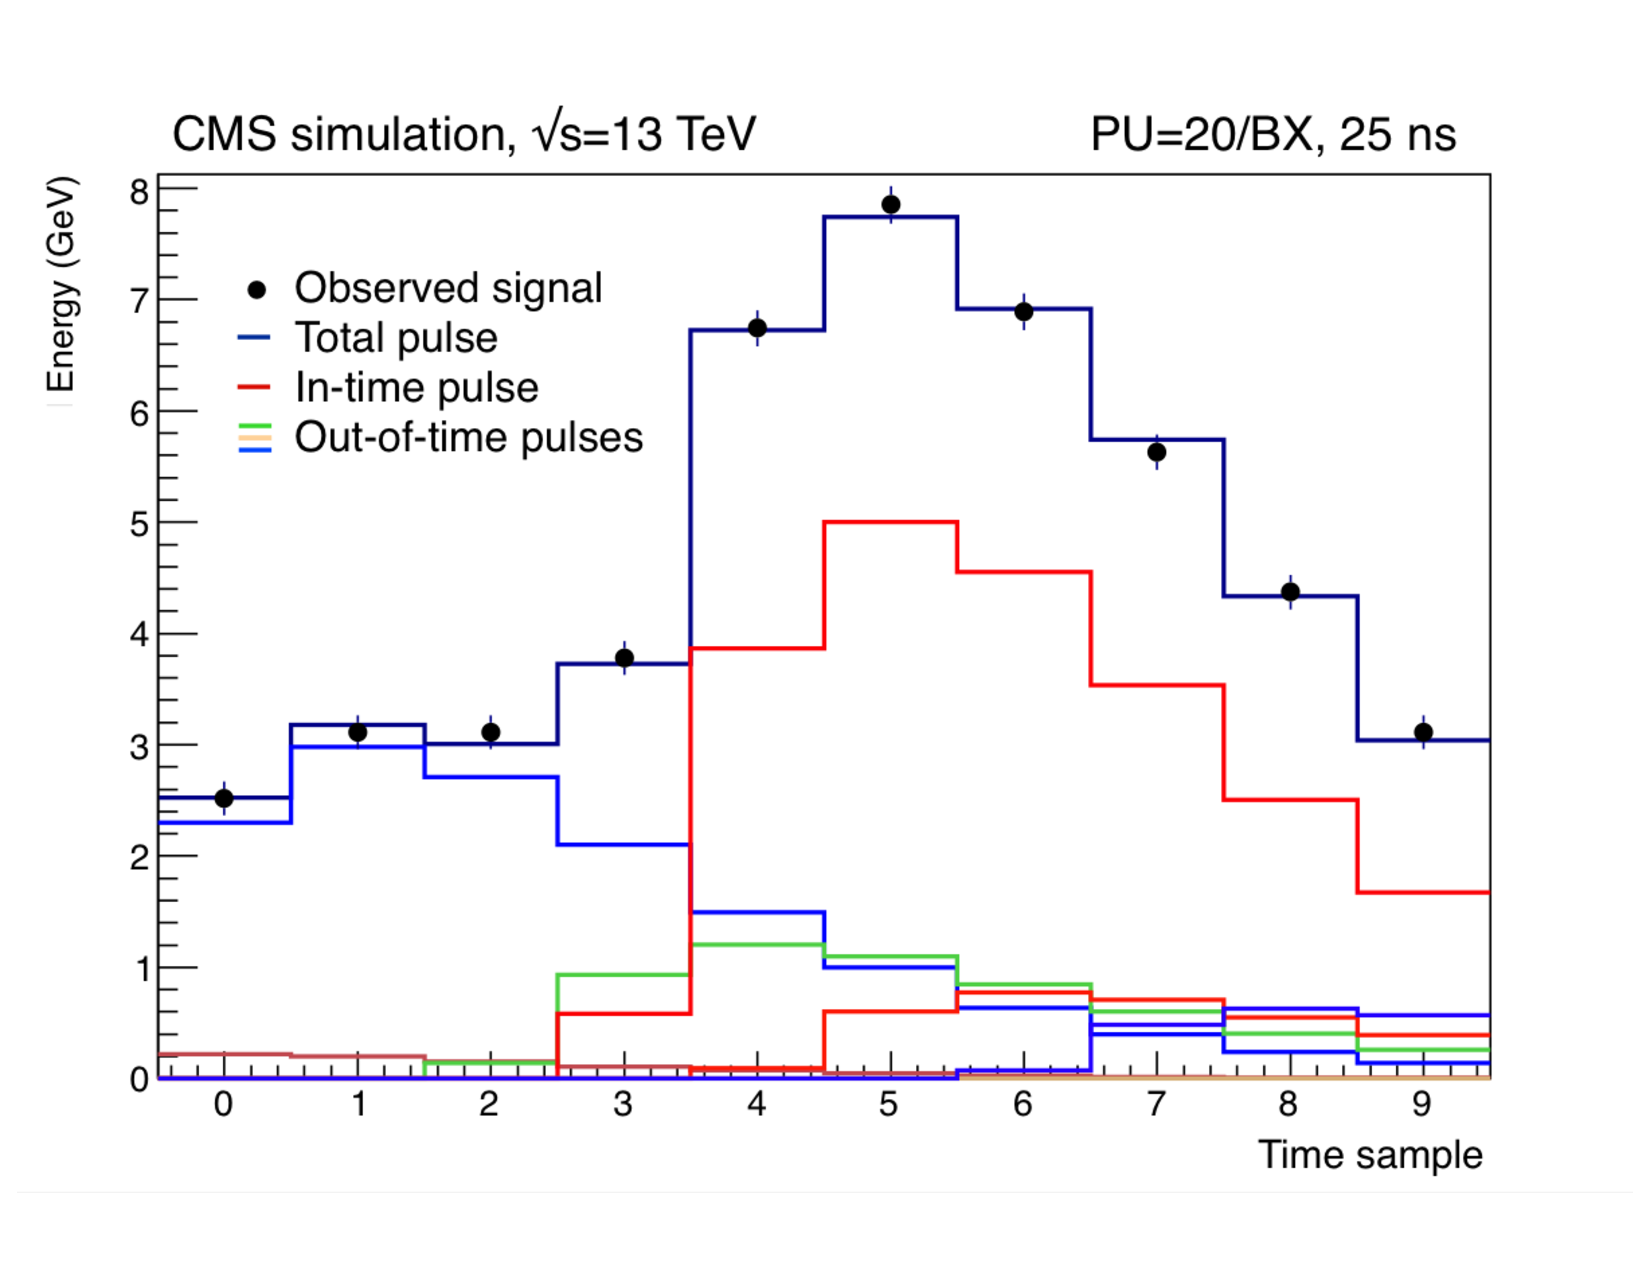
\includegraphics[width=0.45\textwidth]{figures/multifit_pulses}\hfil
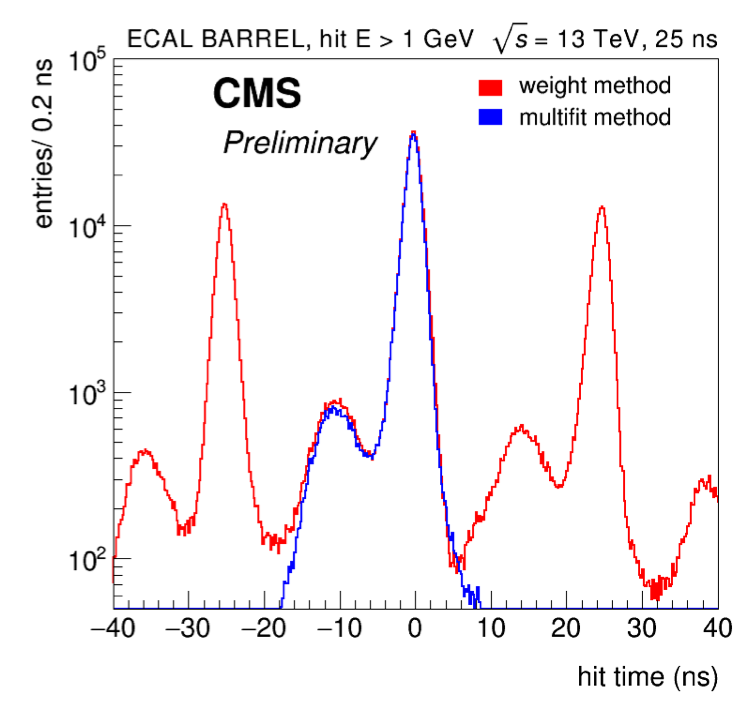
\includegraphics[width=0.45\textwidth]{figures/multifit_oot}\hfil
\caption{(Left) Fitted pulse shapes with the multifit method. (Right) In-time and out-of-time contributions to energy reconstruction with weights method (red) and multifit (blue).}
\label{fig:ecal_multifit}
\end{figure*}


In the multifit method, the pulse shape is reconstructed based on a fit to the time samples, minimizing $\chi^2 = \sum_{i=1}^{10}{\left( \sum_j^MA_jp_{ij} - S_i \right)^2}/{\sigma^2_{S_i}}$. The samples ($S_i$) are fitted with one in-time pulse shape template, plus up to 9  out-of-time templates ($p_{ij}$) times their respective amplitudes ($A_j$). $\sigma_{S_i}$ is noise generated by electronics associated with the crystal readout chain. The OOT templates have the same shape as the in time one, but are shifted in time by multiples of 1 bunch crossing (1 BX = 25 ns), within a range of -5 to +4 BX around the in time signal (BX = 0). The pulse shapes have been measured in early 2015, in special runs in which the LHC delivered isolated bunches (no OOT pile up).

It has been observed in both data and simulation that, with the multifit method, OOT pile up reconstruction is negligible. The energy resolution improvement, with respect to the Run I amplitude reconstruction method, is substantial especially for low $E_{T}$ photons and electrons, given the larger contribution of deposits from pile up to the total energy.


\subsection{Response Monitoring}

Time dependent corrections must be applied to the reconstructed amplitude due to changes in detector response with radiation exposure. These changes in response are due to decreases in crystal transparency and variations in VPT response in endcaps.

The changes in the crystal transparency is due to ionizing radiation creating color centers in the lead tungstate. While the scintillation process remains intact, the amount of light detected by the photodetectors decreases. This effect is partially mitigated through thermal annealing, causing the transparency to increase in the absence of radiation.

A light monitoring system is used to monitor the overall changes in response in the ECAL \cite{ecal_laser}. It consists of a system of lasers (operating at 447 nm, close to the wavelength of peak emission for lead tungstate) that injects light in each ECAL crystal, which is then read by the standard ECAL readout. The change in transparency per crystal ($R/R_0$) is then related to the ratio between reconstructed amplitude and the injected light amplitude ($S/S_0$) through the formula:

\begin{equation}
\frac{S}{S_0} = \left(\frac{R}{R_0} \right)^{\alpha},
\end{equation}
where $\alpha$ has been measured in beam tests and is $\approx 1.5$. $S/S_0$ is then used as a correction factor to account for the response changes.

The light monitoring infrastructure is an integral part of the ECAL DAQ. 
It works alongside of the main data flow, in specific periods in which the LHC bunches are empty (orbit gaps). 
During the orbit gaps, the laser system is shown in different parts of the ECAL barrel and endcaps. 
In about 40 minutes, one reading of the full ECAL is performed. 

The history of response change measurements until the end of 2015 is summarized in Figure \ref{fig:fig_laser}. The changes are up to $6\%$ in the barrel and  reach up to $30\%$ at $|\eta| \approx 2.5$, the limit of the tracker acceptance. For high $|\eta|$ regions, changes are up to $70\%$. The recovery of the crystal response during the long shutdown period is visible. The response was not fully recovered, however, particularly in the region closest to the beam pipe. The monitoring corrections are validated by comparing isolated electron energy as measured by ECAL ($E$) and momentum as measured by the CMS Tracker ($p$), before and after light monitoring corrections. It is seen that the measured corrections bring stability to energy measurements with ECAL.

\begin{figure*}[tbh]
\centering 
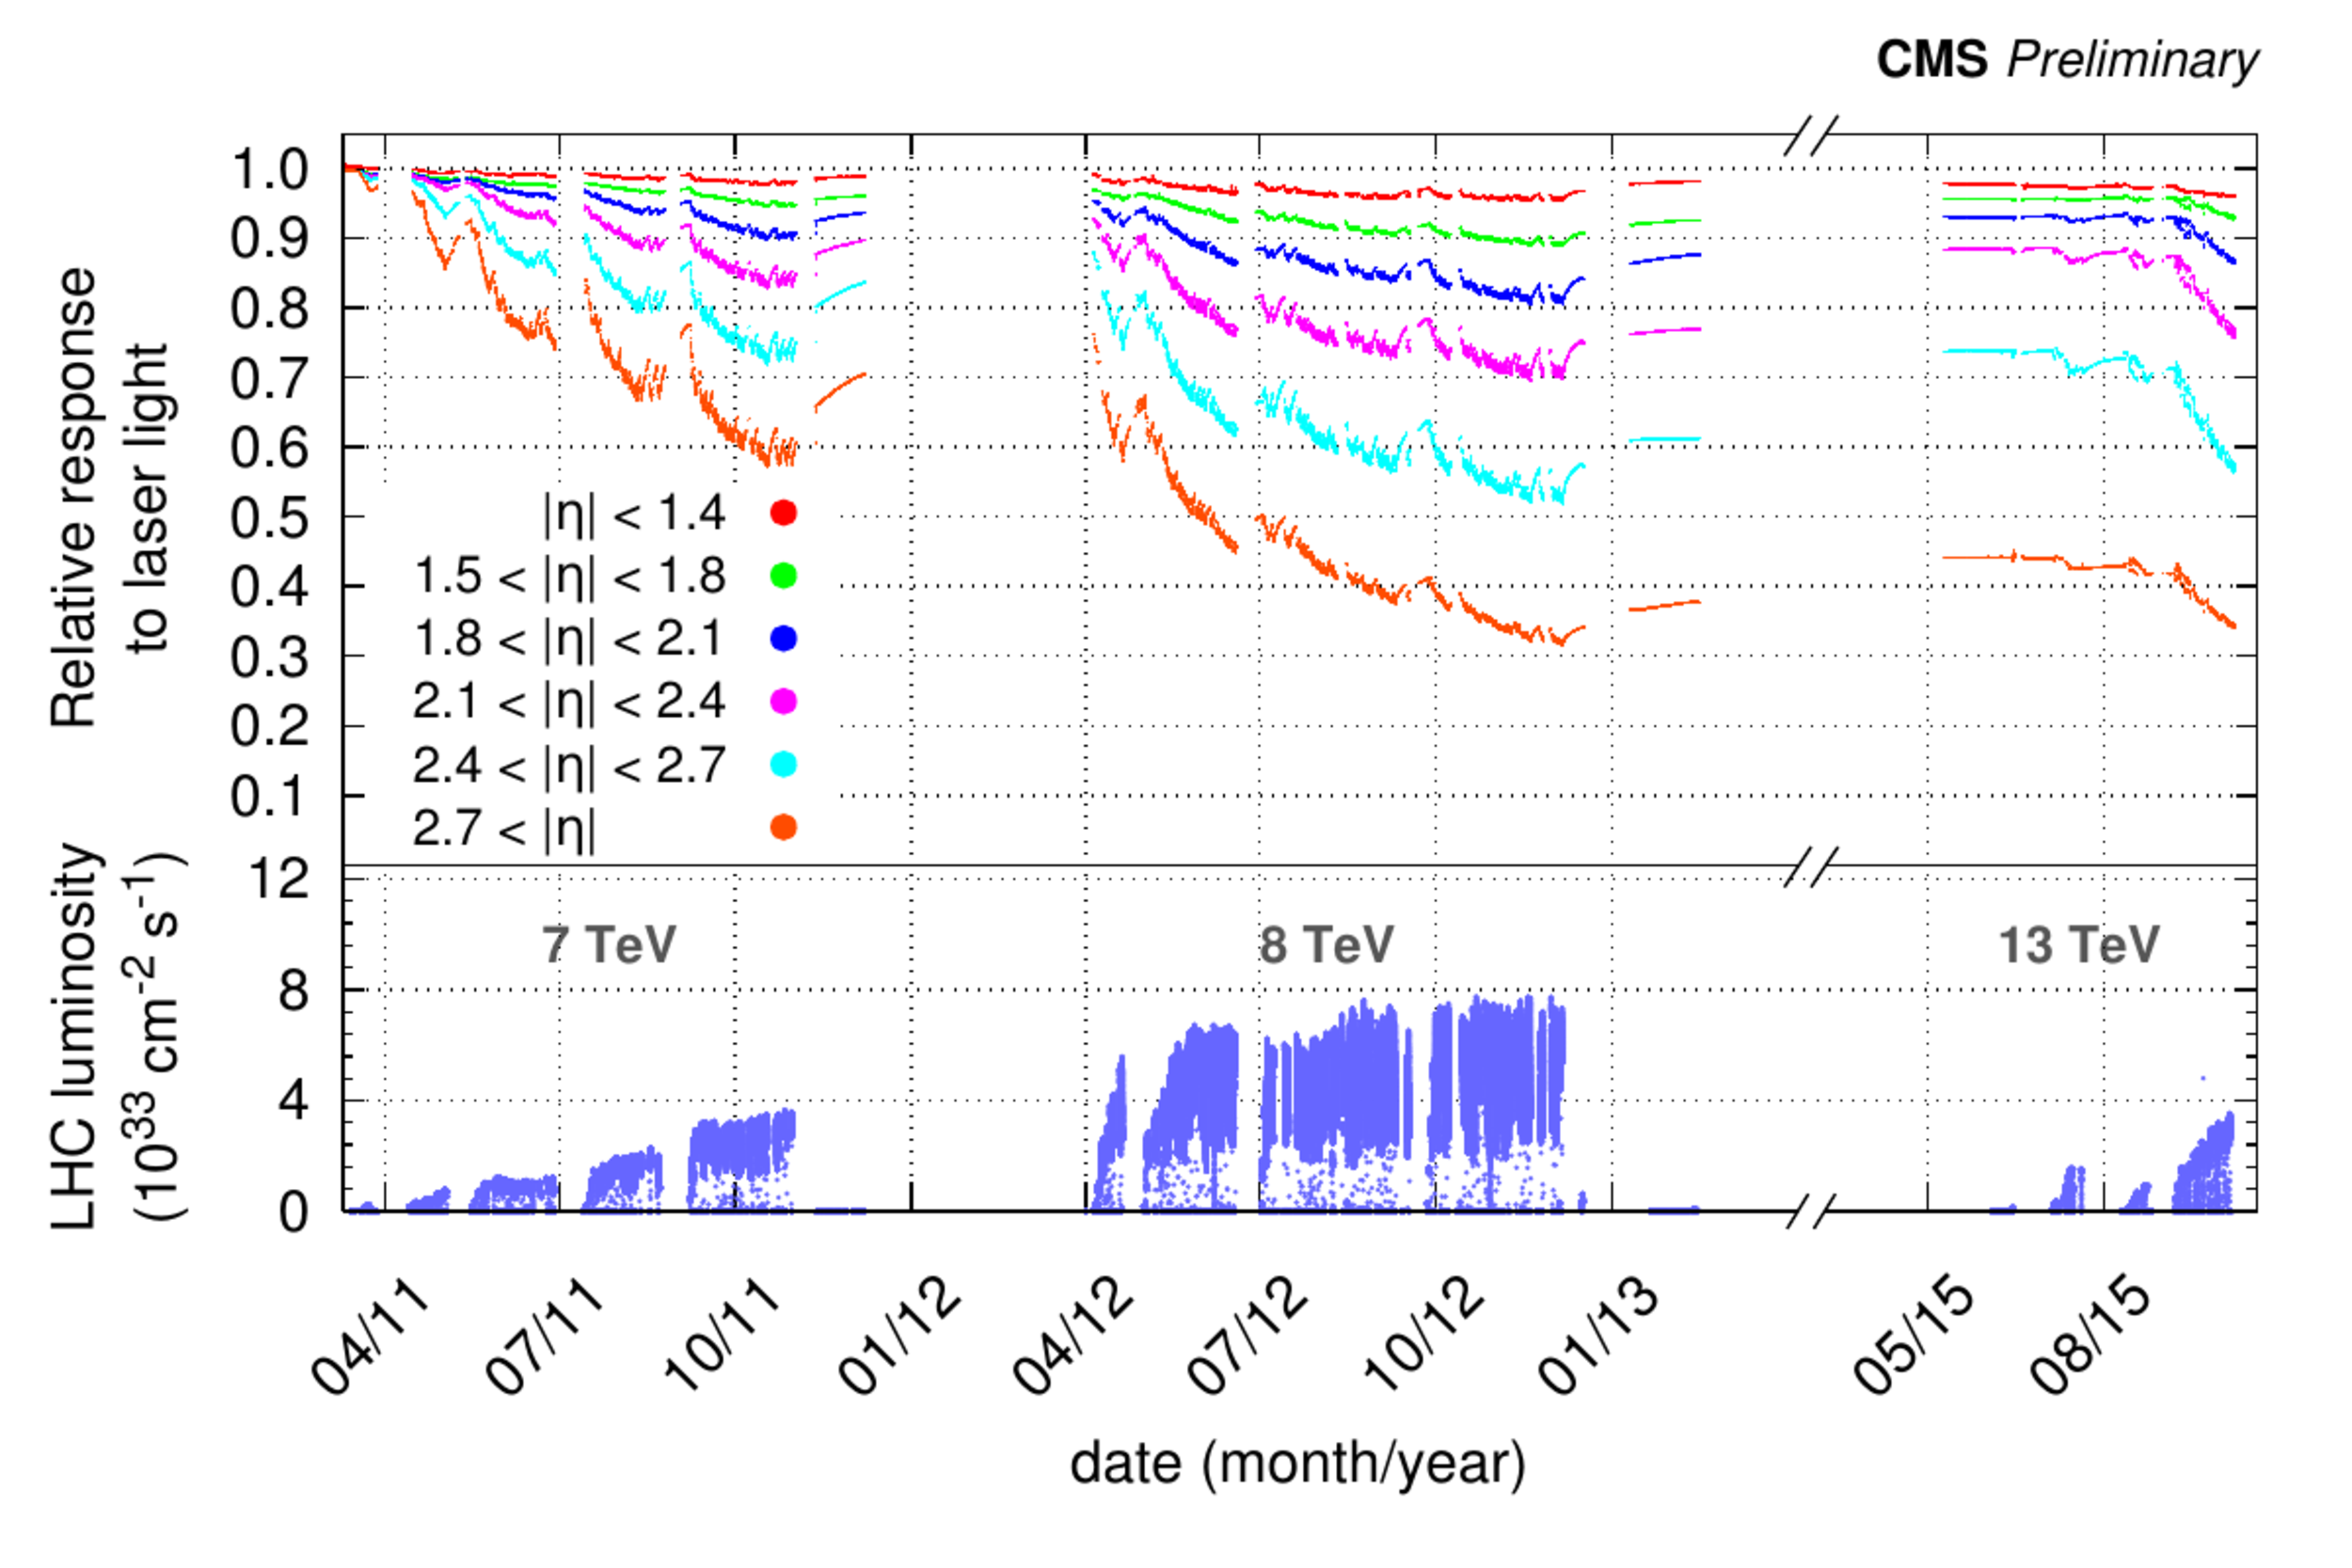
\includegraphics[width=0.8\textwidth]{figures/transparency}\hfil
\caption{History of channel response changes as measured by the light monitoring system.}
\label{fig:fig_laser}
\end{figure*}

In Figure \ref{fig:laser_eop}, it can be seen how the laser corrections impact the stability of the ECAL energy measurement. 
In this plot, the ratio between the energy of an isolated electron as measured by the ECAL (E) and by the CMS Tracker (p) is shown as a function of time. 
Due to the response changes in the crystals and photon detectors, the ratio decreases when left uncorrected. 
After the laser correction is applied, ECAL achieves a stable energy measurement in time.  

\begin{figure*}[tbh]
\centering 
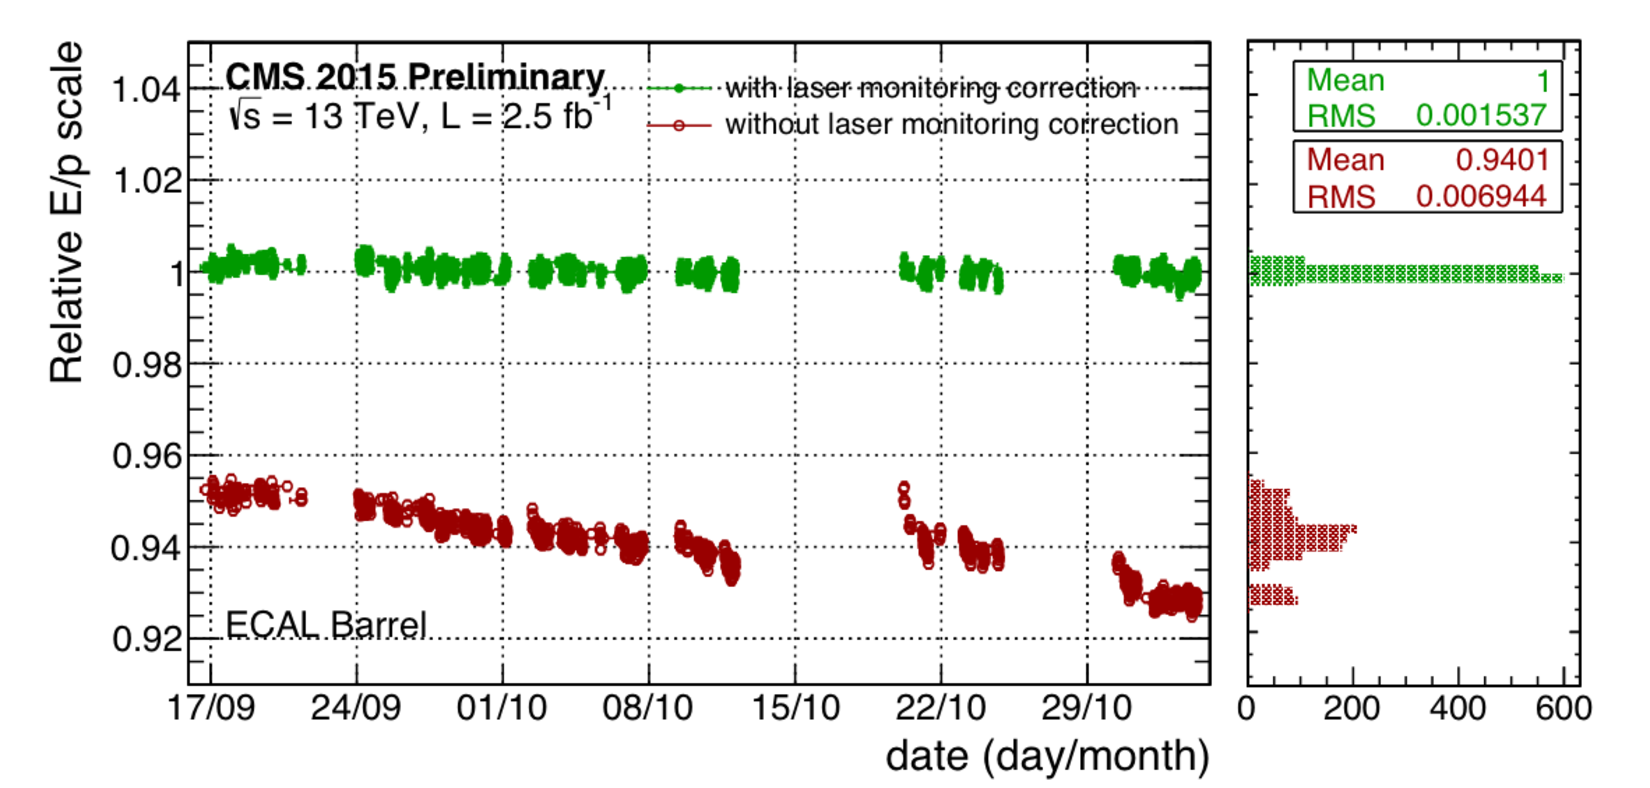
\includegraphics[width=0.8\textwidth]{figures/laser_eop}\hfil
\caption{Stability of electron energy measurement with and without applying laser monitoring corrections.}
\label{fig:laser_eop}
\end{figure*}

\subsection{Intercalibration}

A relative calibration procedure in all ECAL channels is performed to ensure uniformity across the detector. Different and independent methods are used to calculate intercalibration constants (ICs), which are then combined to achieve the desired precision of $<0.5\%$. The final 2015 version of the ICs have been calculated with the full $2.6$ fb$^{-1}$ dataset recorded by CMS with B=3.8 T. The following methods are the same as in Run I \cite{ecal_calib}.

\begin{description}

\item [$\phi$-Symmetry] The $\phi$-symmetry method is based on the expected uniformity of the energy flux along $\phi$ rings (region with fixed $\eta$). The ICs are calculated to correct non-uniformities in this flux. This method was used in 2015 to translate the latest ICs, calculated with the full 2012 dataset, to the 2015 detector conditions. This was done by scaling the 2012 ICs by the ratio between 2015 and 2012 $\phi$-symmetry ICs.

\item [$\pi^{0}/\eta$] The $\pi^0/\eta$ method consists of measuring the invariant mass of these resonances' decays to two photons and maximizing their resolutions by varying the ICs iteratively. This method does not utilize the absolute value of the  $\pi^0$ and $\eta$ resonances not to interfere with the absolute scale calibration. 

\item [E/p] The $E/p$ method employs the same logic as the light monitoring validation method, comparing isolated electron energy and momentum. An iterative method is used to minimize the spread of the $E/p$ distribution.

\end{description}

The combined intercalibration was obtained from the mean of the individual ICs at a fixed value of $\eta$, weighted by their respective precisions. The residual miscalibration of an intercalibration method, which is related to the final method precision, is calculated as the spread of the difference between the method's ICs and the other methods' ICs at a fixed value of $\eta$. 
This residual miscalibration can be seen in Figure \ref{fig:ecal_miscalib}  (left) for the ECAL barrel, where it is shown that the combination of ICs achieves the desired goal of less than $0.5\%$ precision for the central barrel region. 
The overall impact of applying the intercalibration constants and the response monitoring corrections can be seen in Figure \ref{fig:ecal_miscalib} (right), in $Z\rightarrow ee$ events.

\begin{figure*}[tbh]
\centering 
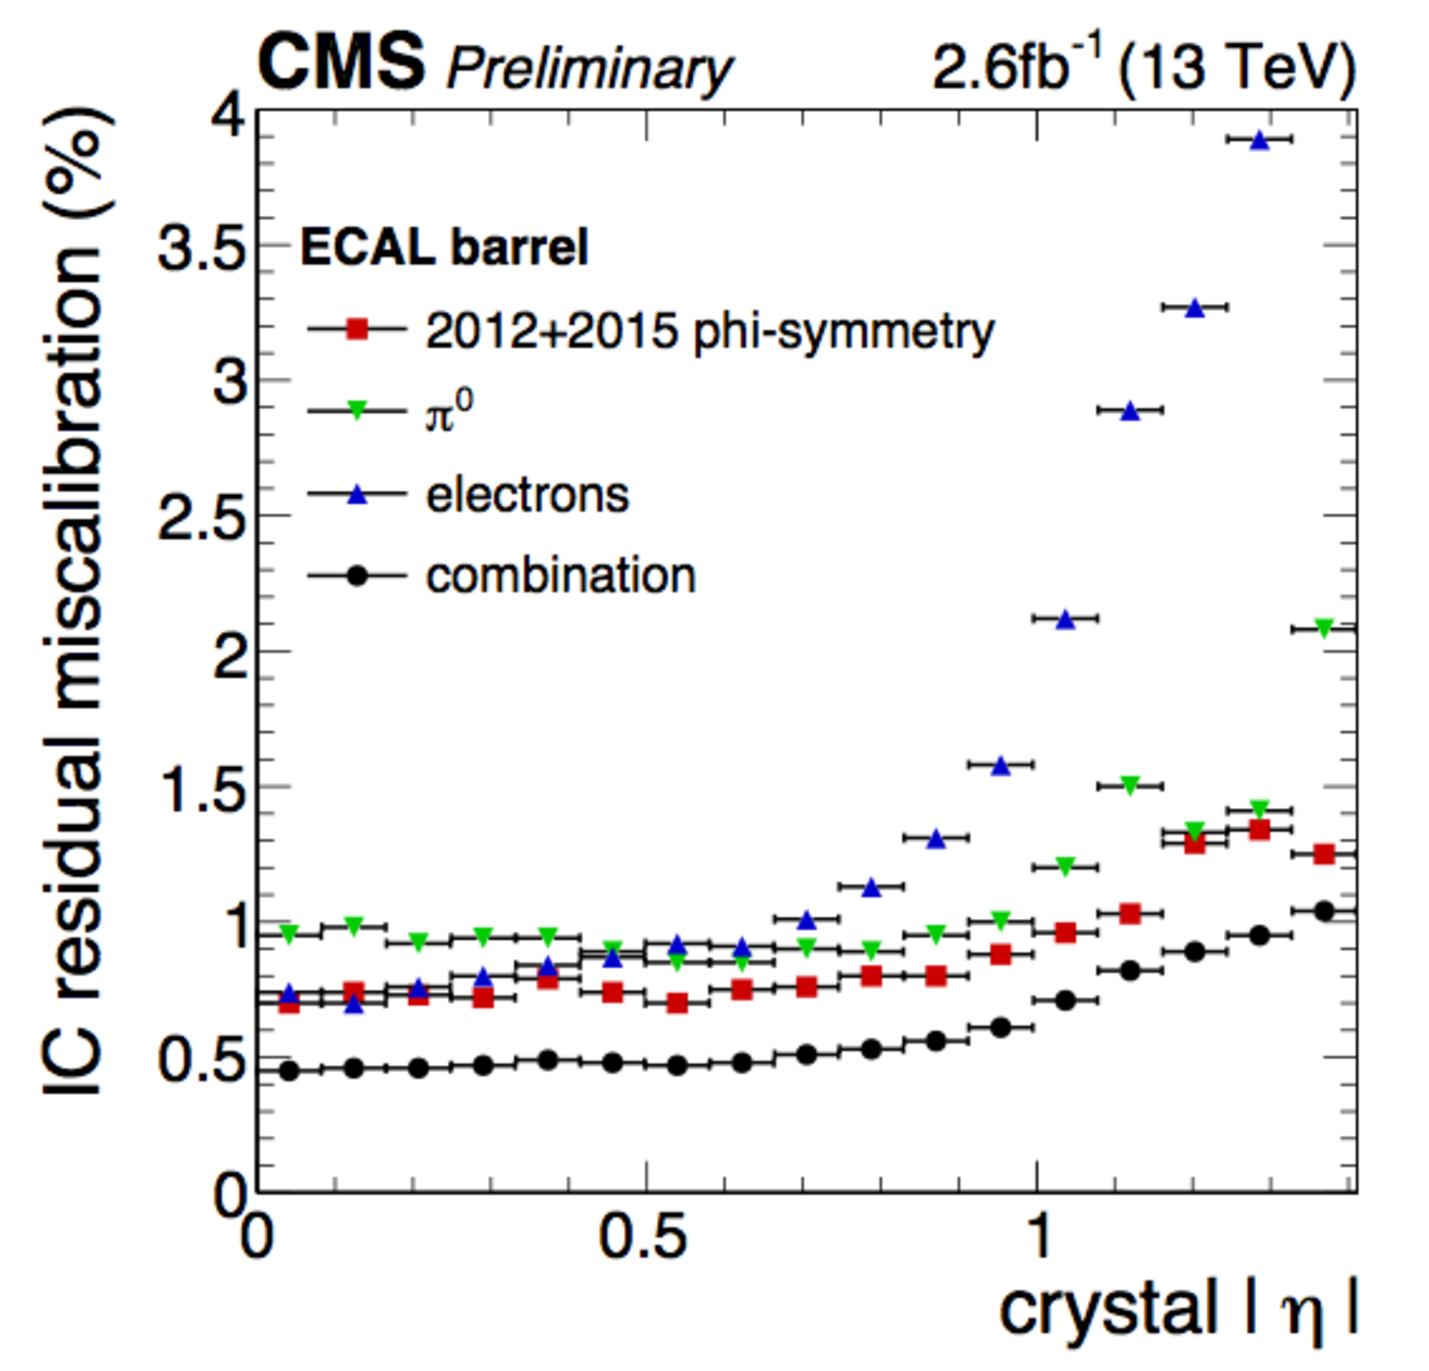
\includegraphics[width=0.45\textwidth]{figures/ecal_miscalib}\hfil
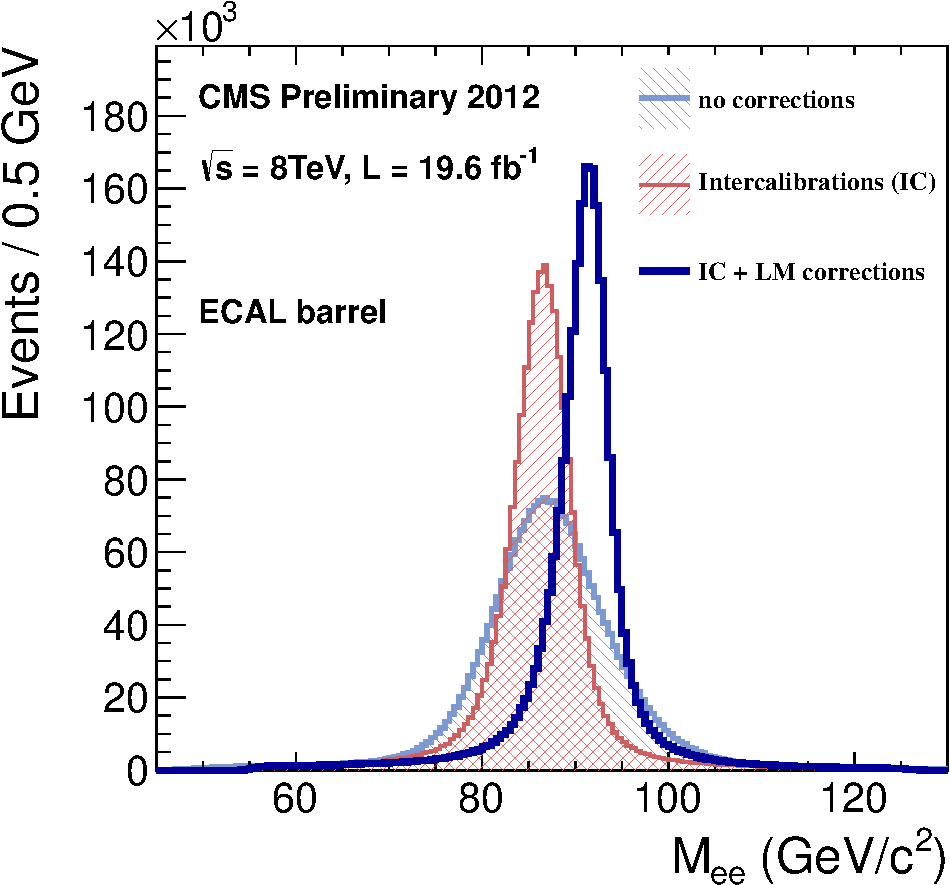
\includegraphics[width=0.45\textwidth]{figures/ecal_ic_lm}\hfil
\caption{Residual mis-intercalibration with the different ECAL intercalibration methods and their combination.}
\label{fig:ecal_miscalib}
\end{figure*}


\subsection{Absolute Calibration}

$Z\rightarrow ee$ events are used both to set the $\eta$ scale and the absolute calibration \cite{ecal_calib}. The first is developed to ensure that  different $\eta$ regions have the same relative response, while the second (done separately for barrel and endcaps) sets the absolute energy scale.

A dedicated calibration was performed with 0 T data taken in 2015 to account for differences in shower shapes in the absence of magnetic field. For example, in 0 T there is no bremsstrahlung radiation outside the main electron cluster deposit, improving the reconstructed energy resolution.

In addition, the calibration was validated with high energy photons and electrons.
%being used in analyses searching for high mass resonances decaying in those particles.
The validation was performed by comparing data and Monte Carlo simulations for high energy electrons from $Z\rightarrow ee$. The calibration was found to be stable to $0.5\%$ ($0.7\%$) for electrons up to $p_{T}=150$ GeV in the barrel (endcap). Possible saturation effects were corrected for with a multivariate technique, but those effects were found to be $<2\%$ for photons arriving from resonance masses less than $1.4$ TeV.

\subsection{High Level Calibrations}

The amount of material in front of ECAL, up to $2X_0$ in the barrel outer regions as seen in Figure \ref{fig:ecal_cluster} (left), produces a high rate of bremsstrahlung radiation from electrons and a high probability of photon conversions. 
To mitigate this effect, a clustering algorithm is used to recombine energy deposits that come from those processes. The cluster energy is corrected via a multivariate technique, separately for photons \cite{cms_egamma} and electrons \cite{cms_electron}. 
It also aims to correct other effects, such as in time pile up. The effect of these high level cluster corrections on the resolution of the $Z\rightarrow ee$ peak can be seen in Figure \ref{fig:ecal_cluster} (right).

\begin{figure*}[tbh]
\centering 
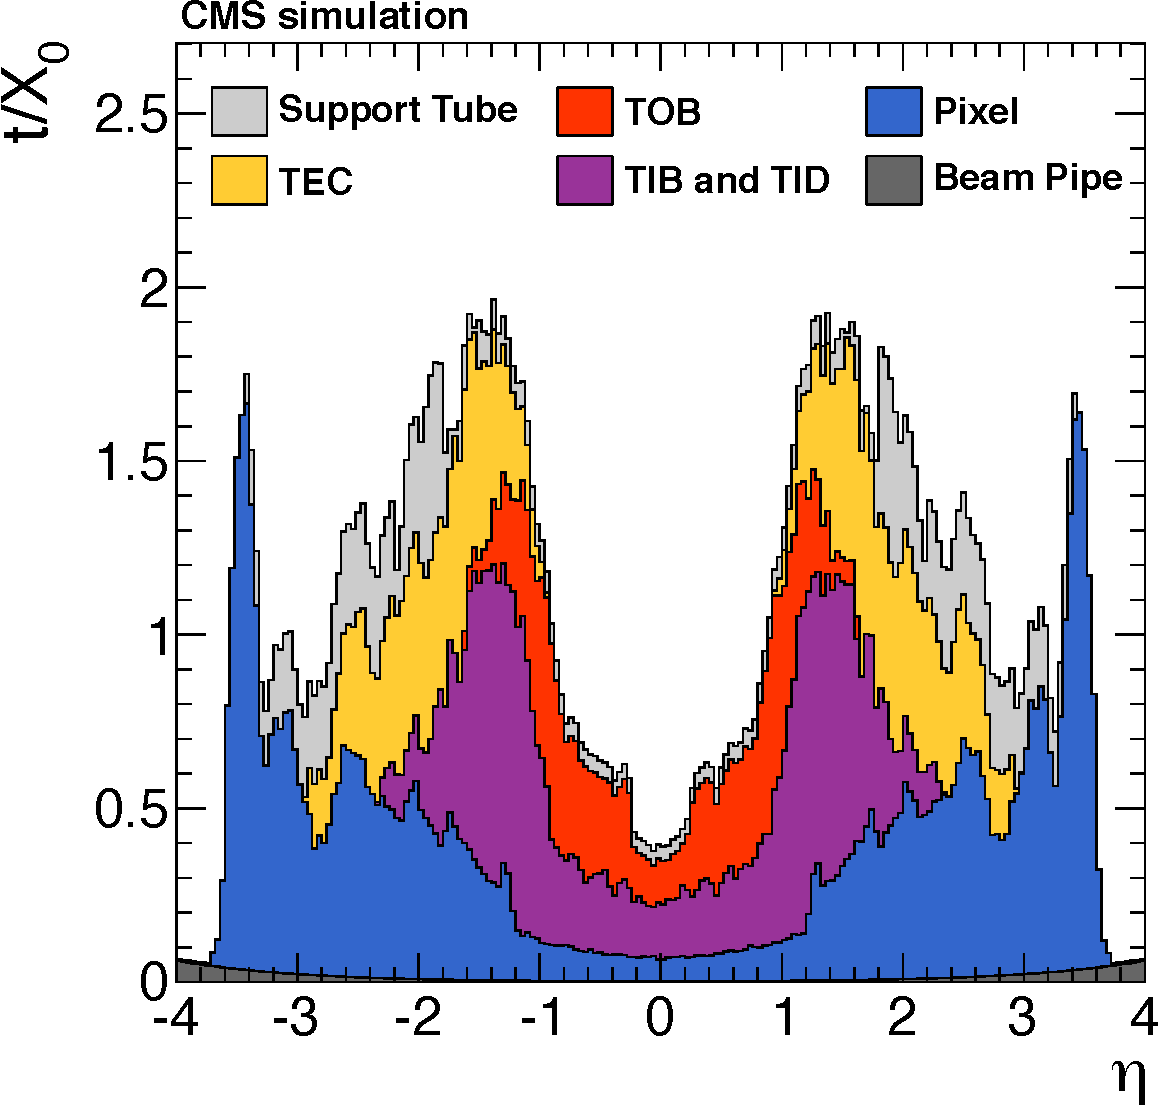
\includegraphics[width=0.45\textwidth]{figures/cms_material}\hfil
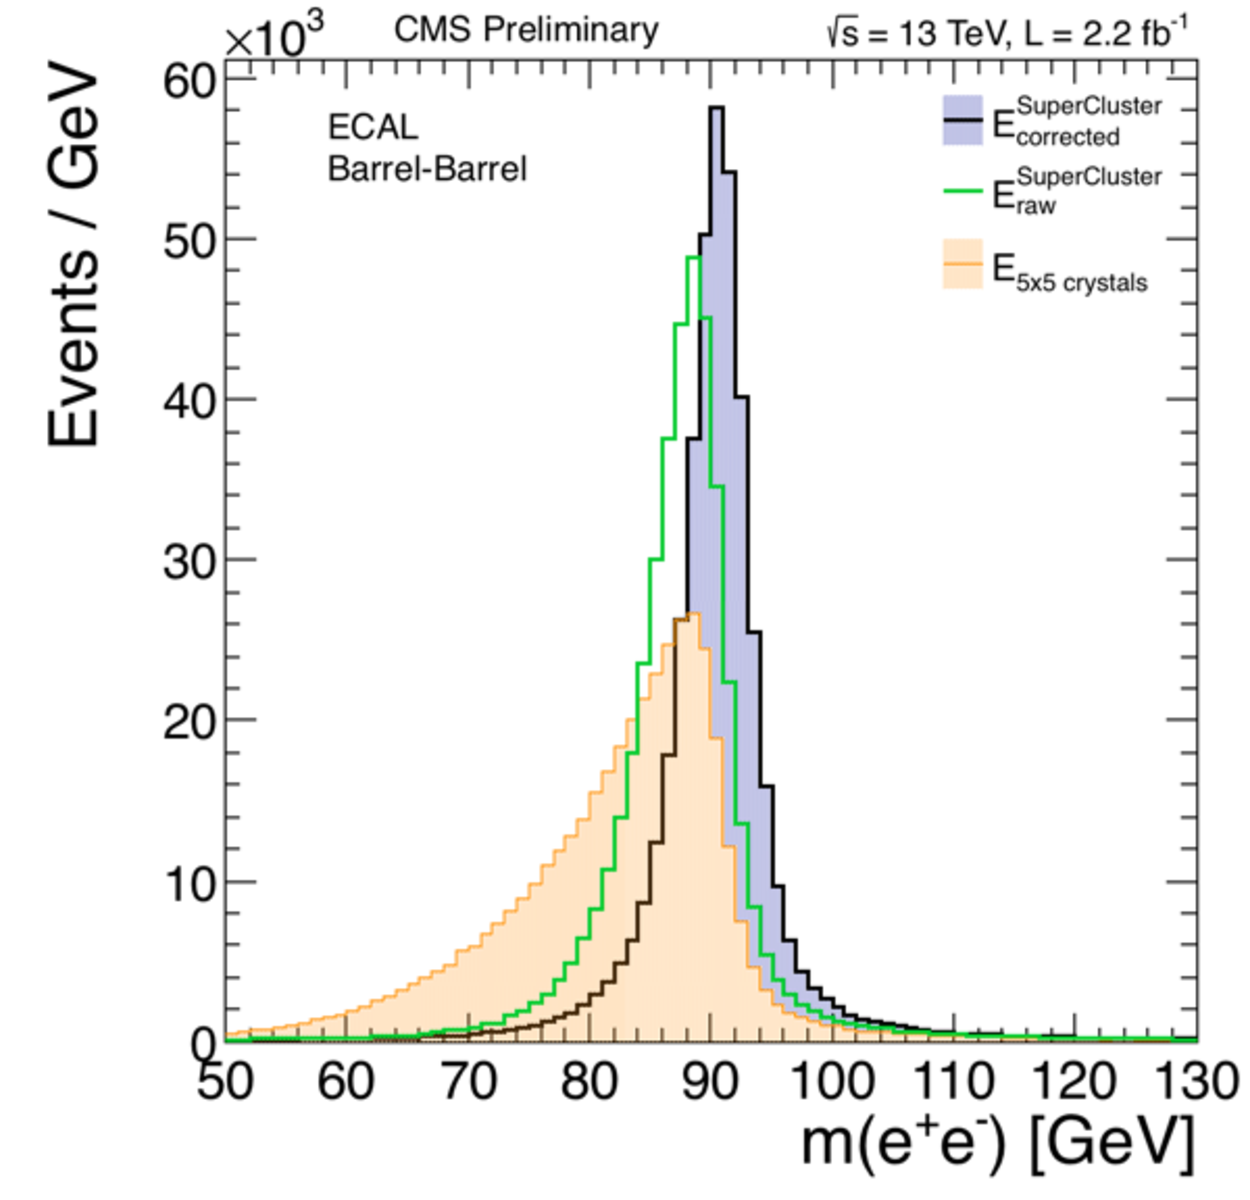
\includegraphics[width=0.45\textwidth]{figures/ecal_clustercorr}\hfil
\caption{Material budget between the ECAL and the collision point on CMS (left). Effect of high level cluster corrections on the resolution of the $Z\rightarrow ee$ peak.}
\label{fig:ecal_cluster}
\end{figure*}


\section{ECAL Energy Resolution}

\subsection{Energy Resolution of a Calorimeter}

The intrinsic energy resolution of an electromagnetic calorimeter can be parametrized in terms of three uncertainty sources, as in the following equation:

\begin{equation}
\left(\frac{\sigma}{E}\right)^{2}  = \left(\frac{A}{E}\right)^{2} + \left(\frac{B}{\sqrt{E}}\right)^{2} + C^{2},
\end{equation}

where the first term on the right-side of the equation is called the noise term, the second is called the stochastic term and the third, the constant term. 
A brief explanation of the physical nature of these uncertainties follows:

\begin{description}
\item [Noise term] The noise term is the contribution to the energy resolution from the electronic noise in the readout chain. In the case of ECAL, this noise comes from the VFE and FE part of the detector, particularly in the light detection phase by the photo-detectors and on the amplification and sampling phase by the MGPA. 

\item [Stochastic term] This contribution to the resolution comes from the physical development of the shower shape inside the detector. For homogeneous detectors, such as ECAL, this term is usually small, since the full shower development is contained within the active medium. 

\item [Constant term] Differently from the other two terms, this one is independent of the energy of the incoming particle in the detector. This uncertainty is related to geometrical and static features of the detector, such as non-uniformities and random instabilities in response that are independent on energy. On ECAL, this contribution is largely mitigated by the intercalibration and laser monitoring calibration.

\end{description}

During the ECAL test-beam commissioning period, these terms were measured directly as: A = 128 MeV, B = 2.8 $\sqrt{\text{GeV}}$ and C = 0.3 \%.

\subsection{ECAL Energy Resolution with Run II data}

The ECAL energy resolution is measured using $Z\rightarrow ee$ events, from an unbinned fit with a Breit-Wigner function convoluted with a Gaussian as signal model. Degradation effects come from the amount of material in front of ECAL and cracks between modules. The resolution, as a function of $\eta$, for low and high bremsstrahlung electrons in the barrel can be seen in Figure \ref{fig:ecal_res}.

\begin{figure*}[tbh]
\centering 
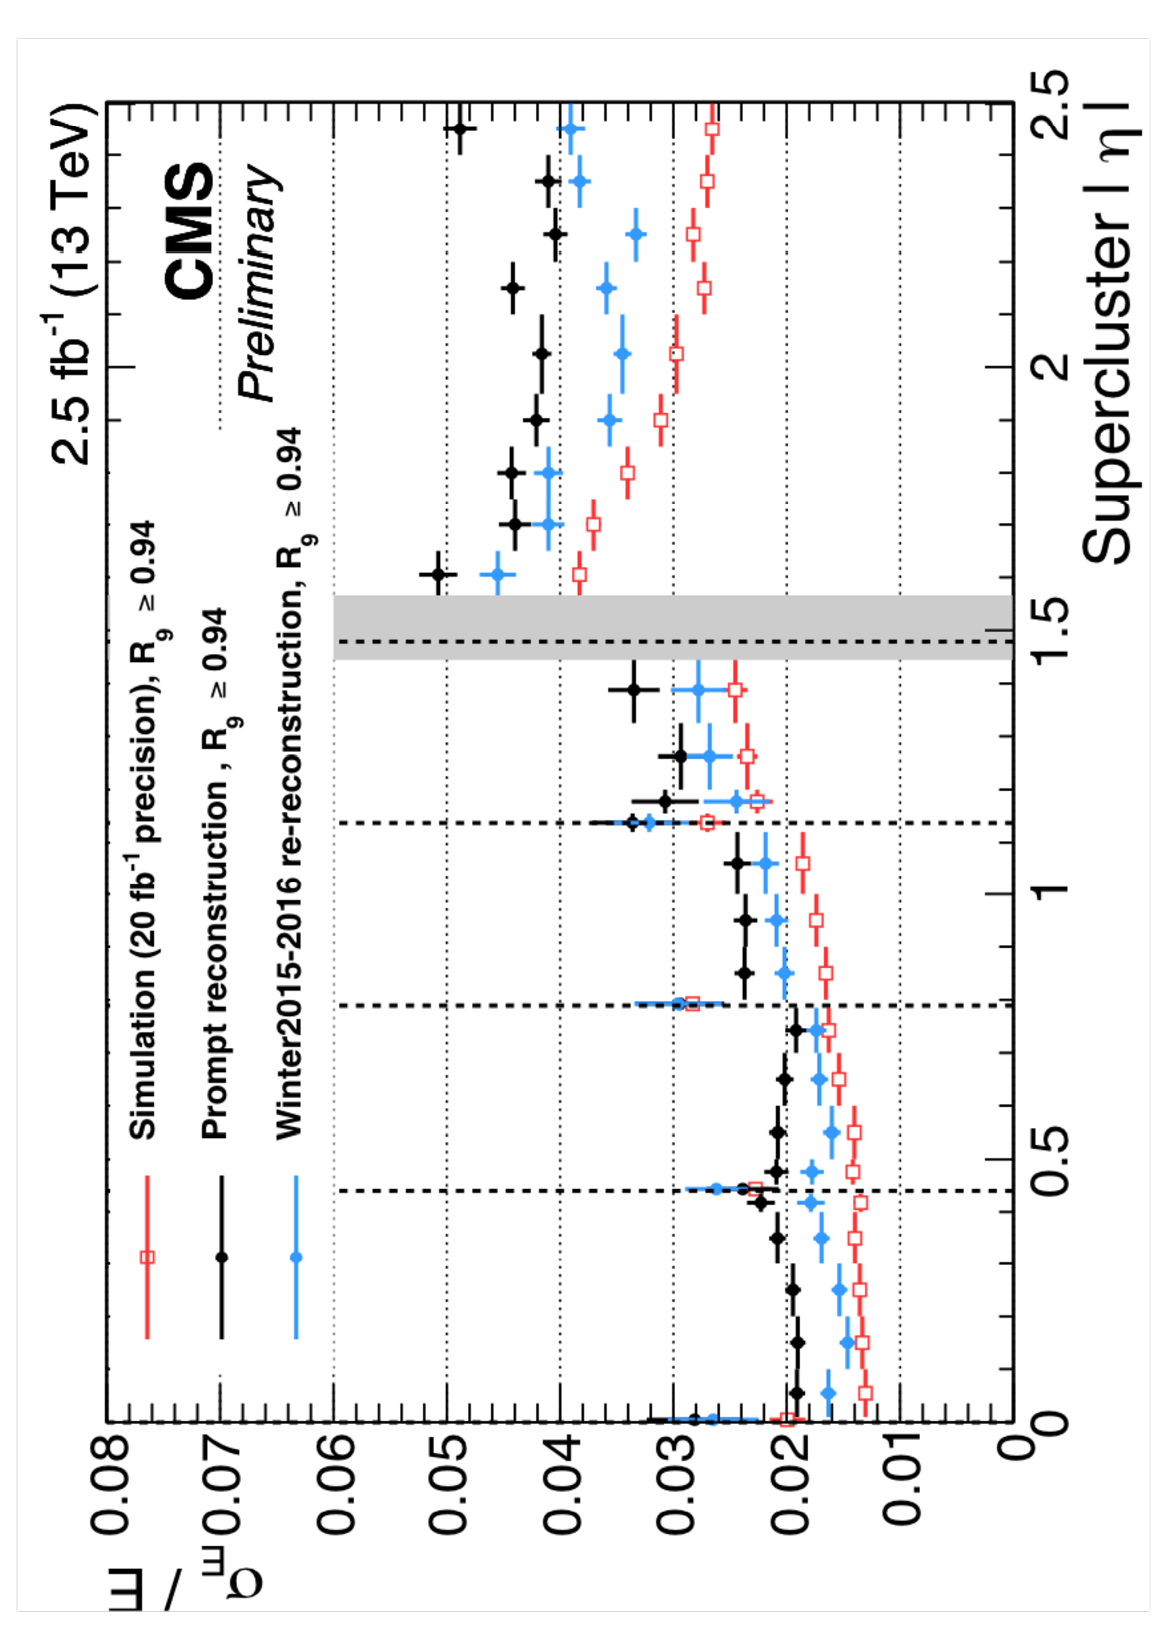
\includegraphics[height=0.45\textwidth, angle=270]{figures/ecal_res_HighR9.pdf}\hfil
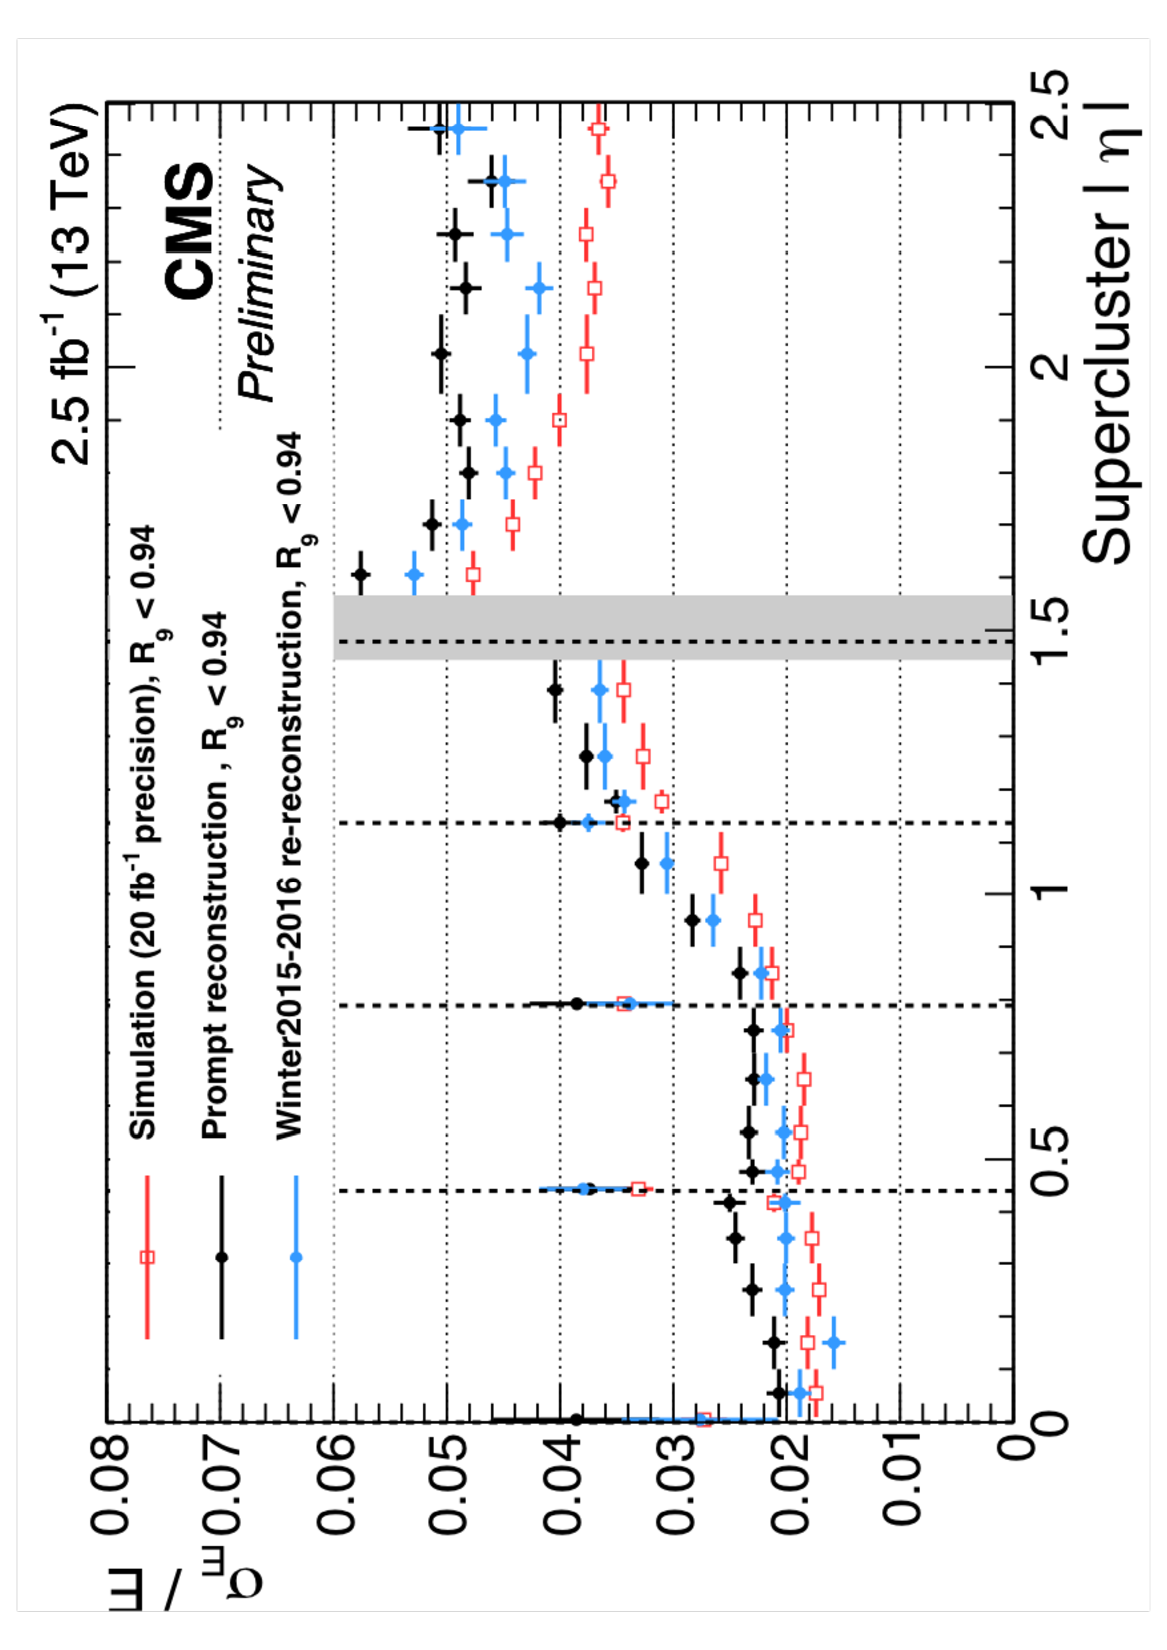
\includegraphics[height=0.45\textwidth, angle=270]{figures/ecal_res_LowR9.pdf}\hfil
\caption{Energy resolution for low (left) and high (right) brehmsstrahlung $Z\rightarrow ee$ electrons as a function of $\eta$.}
\label{fig:ecal_res}
\end{figure*}


The energy resolution achieved with reprocessed data, which includes the latest intercalibration and calibration constants derived with 2015 data, achieves a resolution that is less than 2$\%$ for $Z\rightarrow ee$ low bremsstrahlung electrons in the central barrel region.
%The energy resolution achieved using the latest 2015 calibration constants is less than $2\%$ for low bremsstrahlung electrons in the barrel.
The reprocessed data is especially better performing in the endcaps, when comparing to processed data with 2012 values for intercalibration and calibration. When ported to physics analysis, this energy resolution implies, for example, in a $\sigma_{eff}/M_h \approx 1.5\%$ (from simulation) in the $H\rightarrow\gamma\gamma$ analysis, where $\sigma_{eff}$ is the smallest interval in $M(\gamma\gamma)$ with $68.5\%$ coverage \cite{cms_hgg_15}.


\section{The CMS ECAL Barrel Upgrade}
\subsection{The High Luminosity LHC}

The performance of the Large Hadron Collider, and the physics program carried by ALTAS and CMS, has started remarkably. With the discovery of the Higgs boson in 2012, and the expected 40 fb$^{-1}$ to be delivered in 2016 with record high instantaneous luminosity, the program has exceeded experimental expectations. 
The current LHC setup, with bunch spacing of 25 ns and peak instantaneous luminosity of the order of $10^{34}$ cm$^{-2}$s$^{-1}$, is expected to deliver around 300 fb$^{-1}$ until the end of 2022, when the Long Shutdown 3 (LS3) is planned to start.

During LS3, which is planned to last until 2025, the LHC is expected to replace the quadrupoles that focus the beam for ATLAS and CMS. Additionally, upgrades will be performed to optimize the bunch overlap at the interaction region. These improvements are expected to allow the LHC peak luminosity to reach $2\times10^{35}$ cm$^{-2}$s$^{-1}$ (High Luminosity LHC, HL-LHC). 
The full HL-LHC of around 3000 fb$^{-1}$ will open a brand new physics program at the LHC, involving precise measurements of the Higgs properties and rarer standard model phenomena, such as the standard model Higgs pair production. 

The new LHC configuration will also bring new experimental challenges. With the increased peak luminosity, a higher dose of radiation will be reaching the inner detectors of ATLAS and CMS, causing unrecoverable losses of efficiency in tracking reconstruction and calorimetry, for example. It will also challenge the online performance of the detectors, forcing the trigger systems to cope with higher event rates. To recover its performances to comparable or higher levels of the previous data taking periods, CMS have planned hardware upgrades to be deployed during LS3 \cite{cms_upgrade}.


\subsection{ECAL Electronics Upgrade}

As mentioned in the previous section, the impact of incoming radiation on ECAL is to form color centers on the crystals that damage its transparency. 
With the incoming dose of radiation at the HL-LHC, the endcap crystals are expected to completely lose their transparencies. 
This prompted the CMS community to entirely replace the ECAL endcaps for its HL-LHC upgrade. 
The new ECAL endcap will be based on silicon technology, as a sampling calorimeter (HGCal). 

On the ECAL barrel, the crystals are expected to robustly cope with the incoming dose of radiation (lower than the flux on the endcaps), and will therefore be kept in the detector. 
However, the new levels of radiation will also represent a challenge to the in-detector electronics. 
For example, the dark current on the APDs (the electric current flowing through the photo-detector even in the absence of signal, created by random processes) is expected to increase, given the higher ionizing radiation dosage hitting the detector. 
This dark current is a large contributor to the noise term in the energy resolution formula, specially to homogeneous calorimeters, and upgrades must be devised to keep it under control. 

\subsubsection{VFE Upgrade}

For the HL-LHC upgrade, two ways to mitigate the increased detector noise have been investigated: replacing the VFE and cooling the ECAL crystals and APDs from 18$^{o}$C to 8$^{o}$C. 
The APDs cooling works reducing the dark current expected at high integrated luminosities scenario. 
The downside of this upgrade is the decreased light yields from scintillation from the lead tungstate crystals. 
The VFE upgrade intends to reduce the electronics noise by reducing the shaping time attached to the amplifying process, currently at 40 ns. 
This reduction limits the impact of electronics noise in the amplitude reconstruction, while also allowing for a more precise time resolution measurement with ECAL. 
These improvements can be seen in Figure \ref{fig:ecal_noise_intlumi} (left). 
Figure \ref{fig:ecal_noise_intlumi} (left) also shows that, in the scenario with no HL-LHC upgrades, the noise present on the ECAL barrel would reach levels almost 10 times higher than the current value (1.5 ADC counts). 
The upgrade reduces the noise at 3000 fb$^{-1}$ by a factor of almost 2. 

\begin{figure*}[tbh]
\centering 
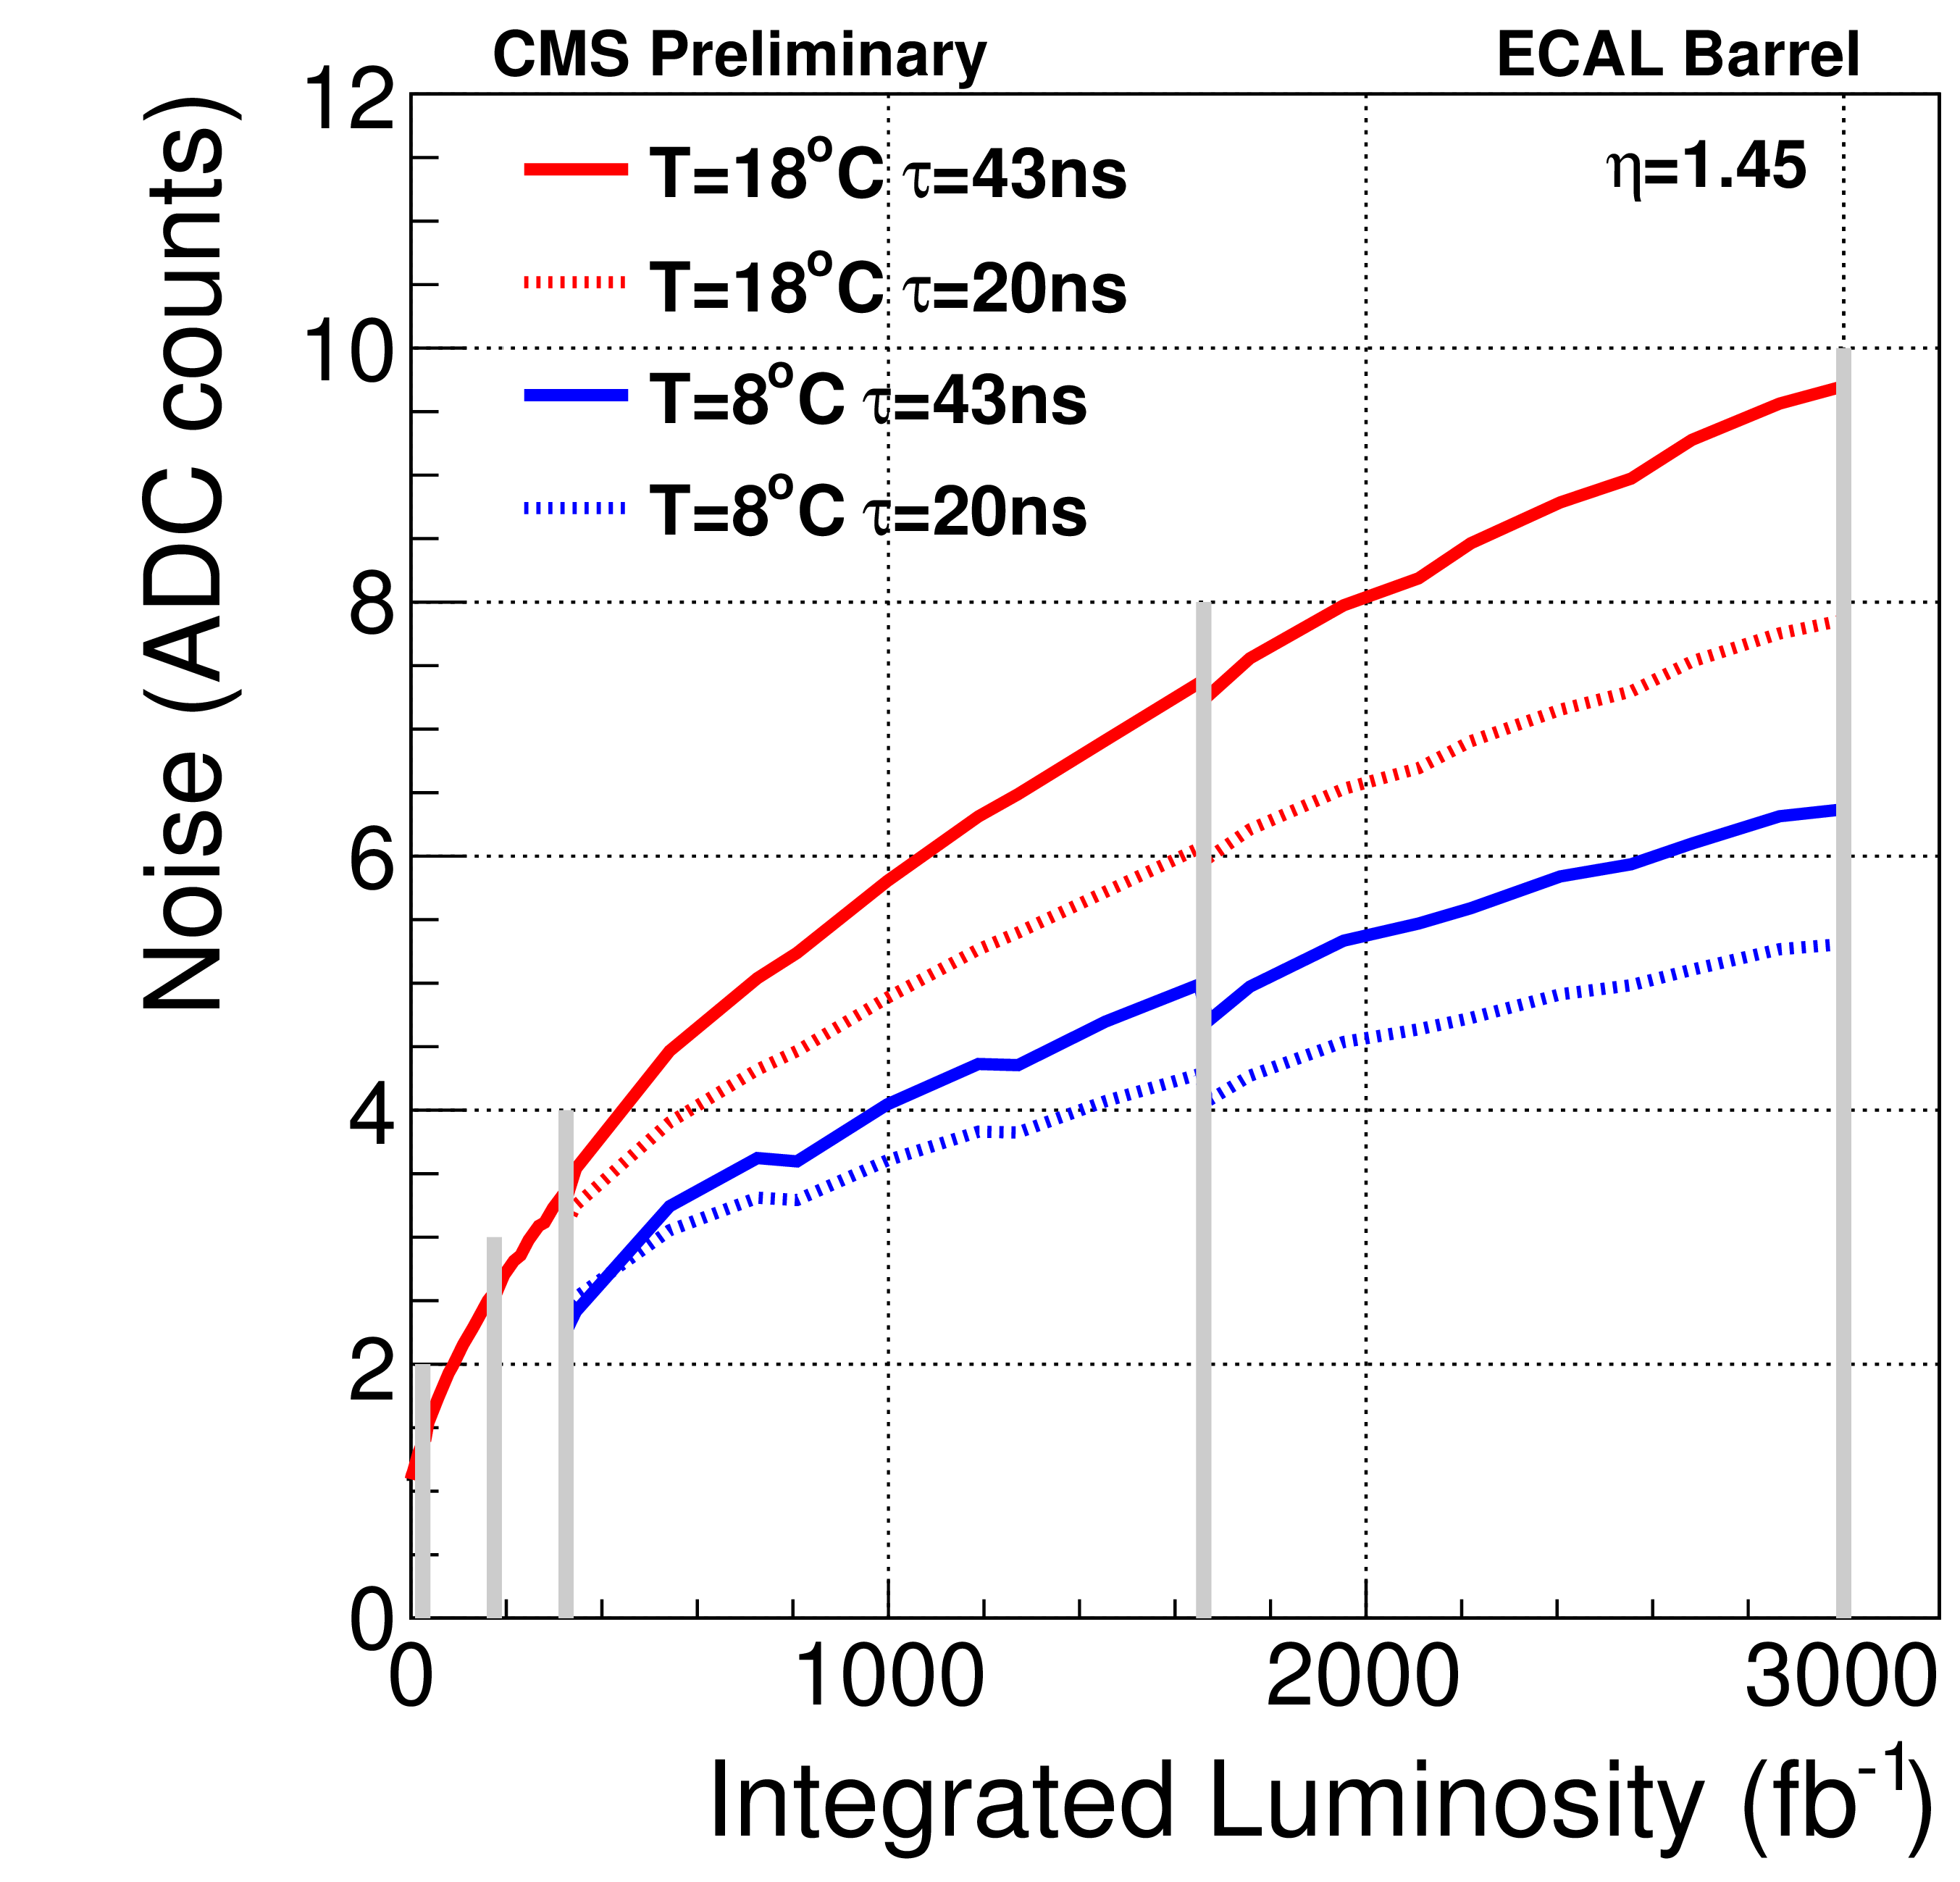
\includegraphics[width=0.45\textwidth]{figures/ecal_noise_intlumi}\hfil
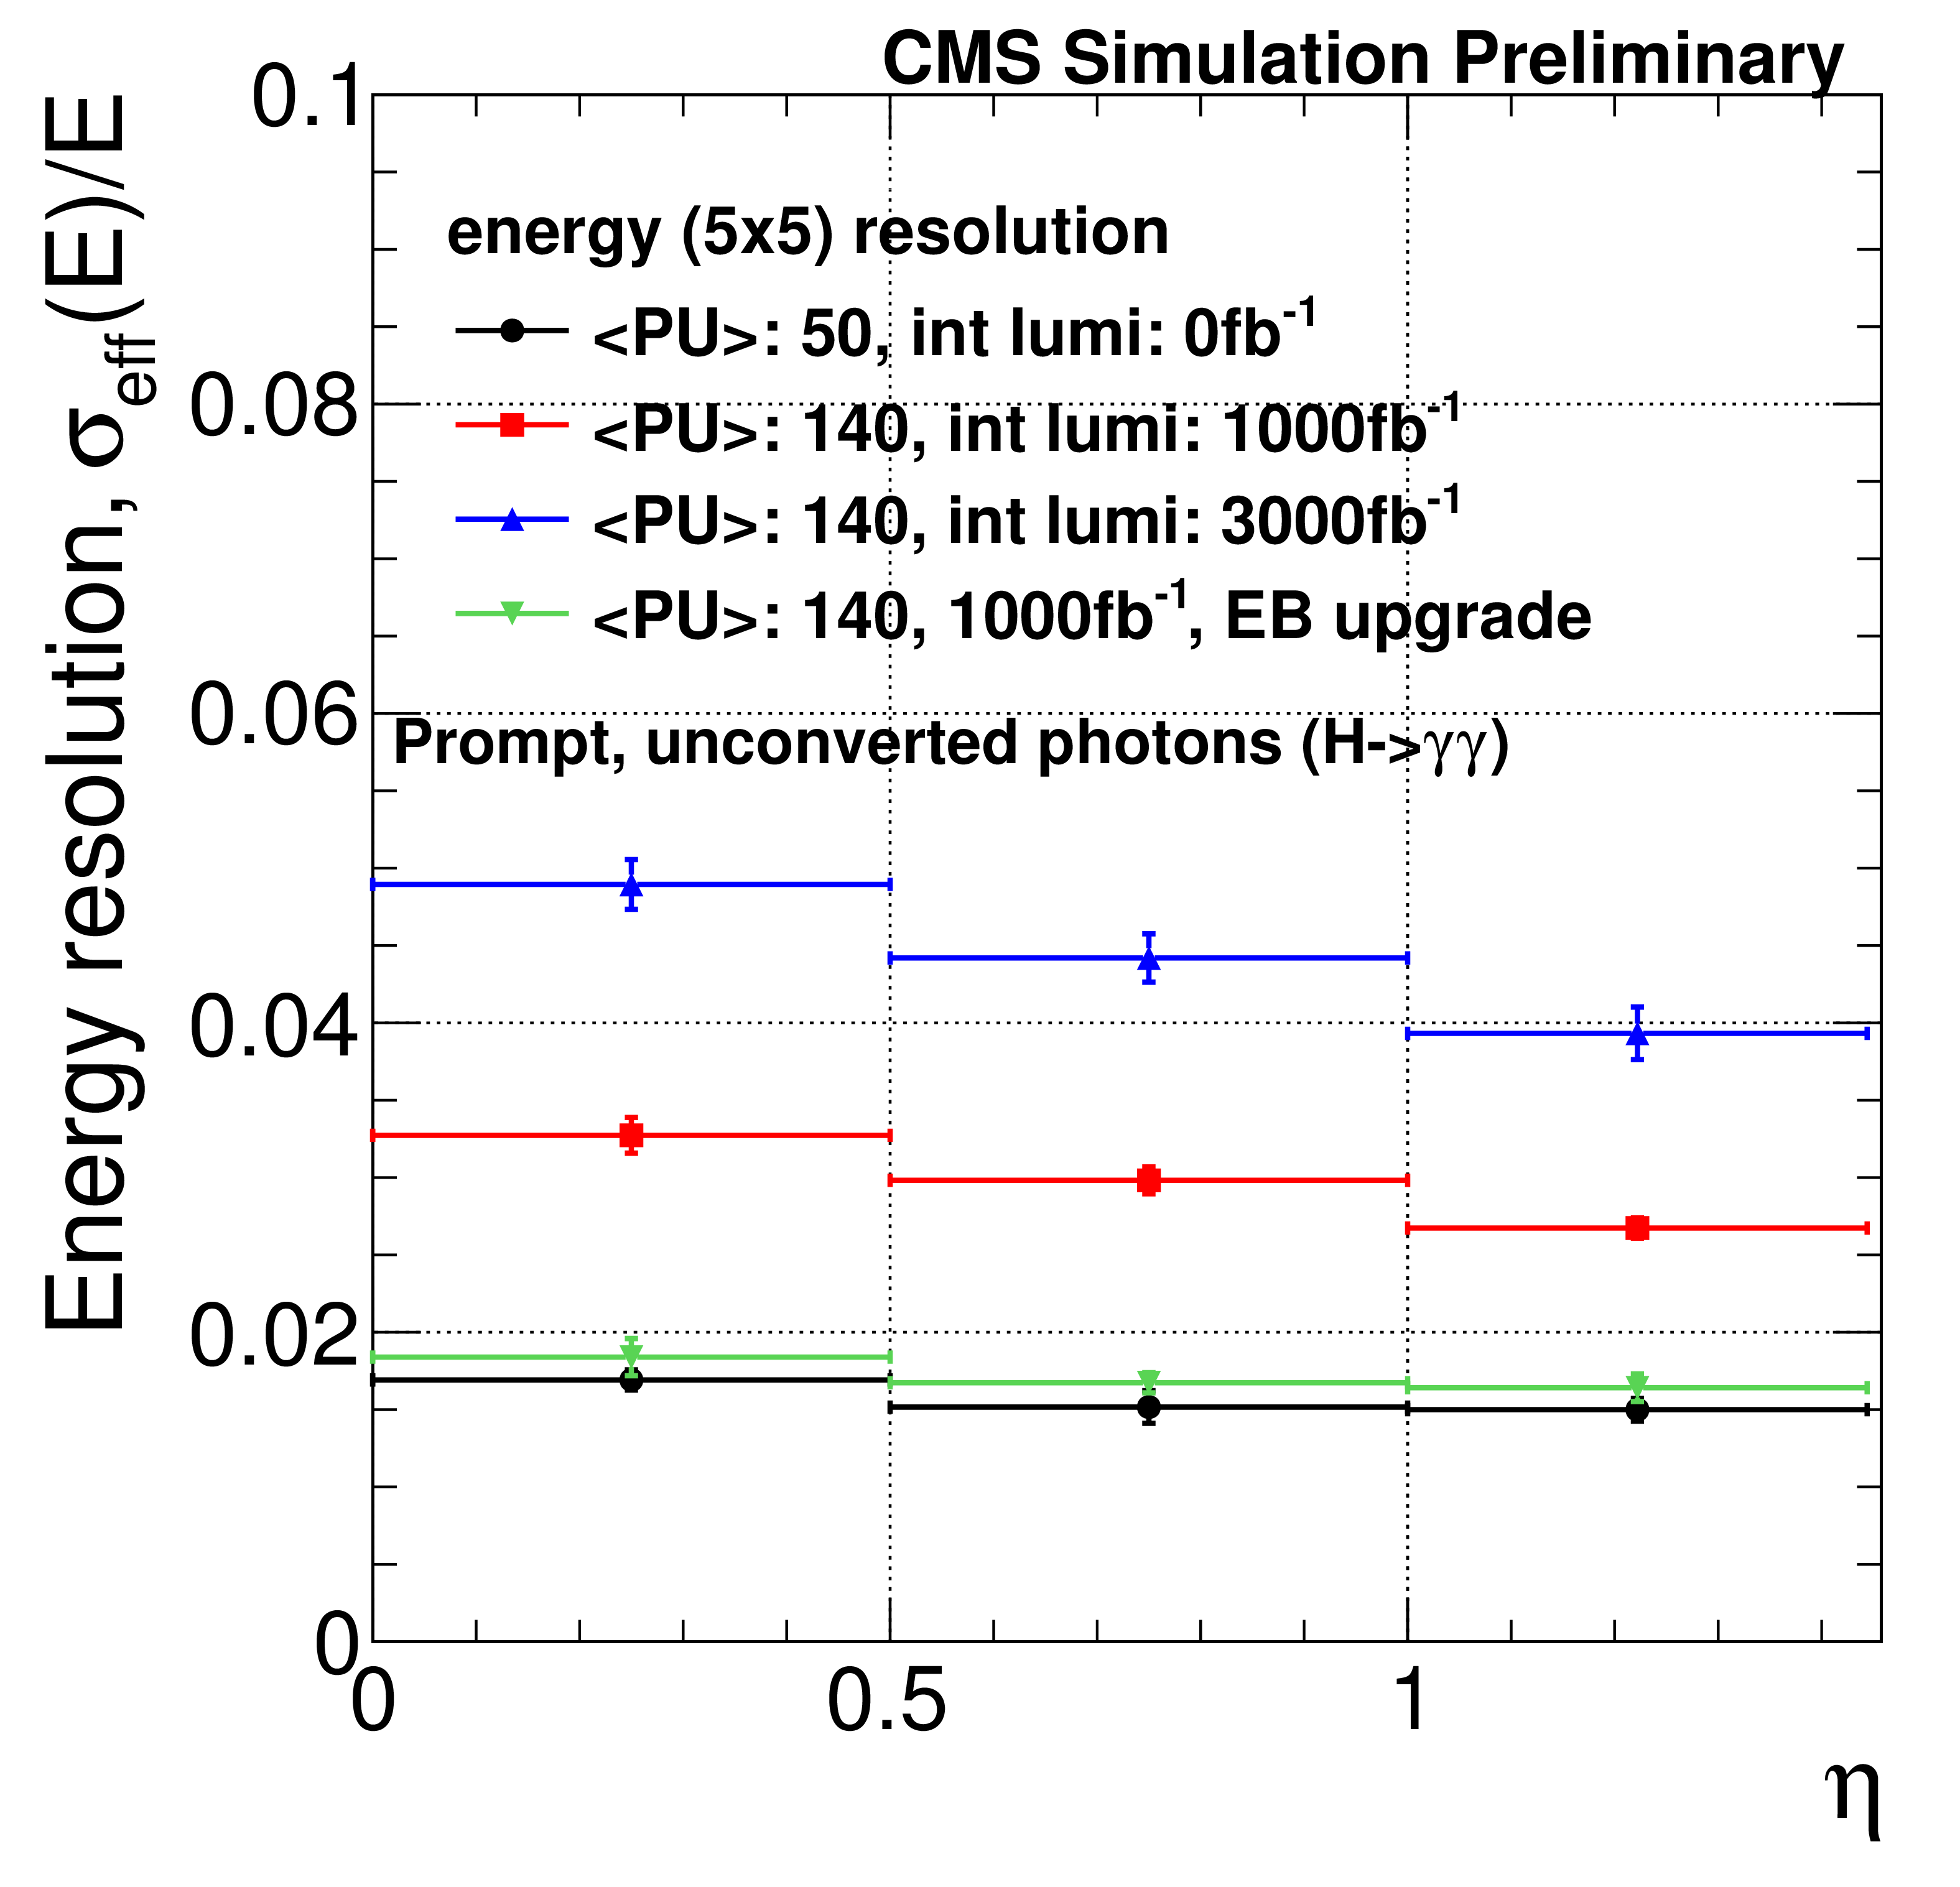
\includegraphics[width=0.45\textwidth]{figures/ecal_upgrade_performance}\hfil
\caption{Noise levels on the upgraded ECAL barrel assuming different upgrade scenarios.}
\label{fig:ecal_noise_intlumi}
\end{figure*}

The noise reduction is translated into physics performance, for example, in $H\rightarrow\gamma\gamma$ searches, as seen in Figure \ref{fig:ecal_noise_intlumi} (right). 
Figure \ref{fig:ecal_noise_intlumi} (right) shows the energy resolution of good quality  $H\rightarrow\gamma\gamma$ photons under different integrated luminosity scenarios, with and without the ECAL barrel upgrade. 

\subsubsection{Trigger Upgrade}

Another important issue arising from the HL-LHC environment is the increase in electronic spikes in the APDs. 
These spikes are created when a high energy hadron hits the APDs directly, without showering in the ECAL crystals. 
This creates an energy discharge in the APD that can fake a signal from a regular particle shower. 
Spikes are problematic when they happen with high frequency because they enhance L1 trigger rates. 
These trigger must then have high energy thresholds in order for the rates to be acceptable by the CMS L1 trigger. 

Another way currently implemented to suppress spikes at trigger level is through coarse geometric variables. 
These variables are computed at the trigger primitive generation step, at the front-end electronics. 
Due to computational limits of the FE boards, these variables use limited information about the crystal array. 
This can be changed if the TP generation happened at the off-detector electronics instead. 
However, this would mean transmitting the full crystal information of the whole ECAL to the off-detector electronics at collision rate (40 MHz). 
By the time of the ECAL commissioning period, the data links could not cope with such requirements, and so the trigger tower based TP generation was implemented. 

One of the foreseen ECAL barrel upgrades is aimed at mitigating those constraints by moving the TP generation step to the off-detector electronics. 
New data links will be used to transmit all crystal data directly from the VFE, instead of being stored waiting for an L1A. 
With extra computing power based on modern FPGAs, new strategies can be investigated to reduce the impact of spikes at L1 trigger level. 
One of these strategies is based on analyzing the signal pulse shape coming from the crystals. 
Given the smaller shaping time from the upgraded VFE, differences in pulse shapes from regular energy showers and spikes can become visible for ECAL.
